\documentclass{report}
\usepackage{fancyhdr}
\usepackage{titlesec}
\usepackage[margin=1in]{geometry}
\usepackage{listings}
\usepackage{color}
\usepackage{graphicx}
\usepackage{amsmath}
\usepackage{booktabs}
\usepackage{amssymb}
\usepackage{algpseudocode}
\usepackage{algorithm}
\usepackage{verbatim}
\usepackage{pdfpages}
\usepackage{placeins} % Add this line
\usepackage[
backend=biber,
sort=ynt
]{biblatex}

\addbibresource{bibliography.bib}

\renewcommand*\thesection{\arabic{chapter}.\arabic{section}}
\renewcommand*\thesubsection{\arabic{chapter}.\arabic{section}.\arabic{subsection}}
\renewcommand*\thesubsubsection{\arabic{chapter}.\arabic{section}.\arabic{subsection}.\arabic{subsubsection}}
\definecolor{dkgreen}{rgb}{0,0.6,0}
\definecolor{gray}{rgb}{0.5,0.5,0.5}
\definecolor{mauve}{rgb}{0.58,0,0.82}
\setcounter{secnumdepth}{3}

\titleformat{\section}
{\LARGE \textbf{\thesection}~}
{}
{0em}
{\bfseries}

\titleformat{\subsection}
{\Large \textbf{\thesubsection}~}
{}
{0em}
{\bfseries}

\titleformat{\subsubsection}
{\hspace{0.3em} \large \textbf{\thesubsubsection}~}
{}
{0em}
{\bfseries}

\titleformat{\subsubsubsubsection}
{\normalsize \textbf{\thesubsubsubsection}~}
{}
{0em}
{\bfseries}

\renewcommand{\maketitle}{
\pagenumbering{gobble}
\begin{center}
\huge
\textbf{Major Project} \\[1em]
\huge
\textbf{Design Document} \\[2em] % Adjust space between the two lines as needed



\vspace{1em}

on

\vspace{1em}


\vspace{1em}
\LARGE
\textbf{EduFlash : Interactive Learning Platform}




\hspace{1em}

Submitted by\\
\vspace{1em}

\Large
Sai Anand K (20221074)\\
Shiva Surendran (20221076)\\
Sidharth Thejas (20221079)\\
S R Angelo Antony (20221081)\\
\end{center}
}
\vspace{1em}
\begin{document}
\begin{center}
\title{EduFlash : Interactive Learning Platform}
%\topskip0pt
\vspace*{\fill}

\maketitle

\begin{center}
\large
In partial fulfilment of the requirements for the award of degree of Bachelor of Technology in Computer Science and Engineering.

\begin{figure}[hbtp]
\centering

\includegraphics[scale=0.6]{cusatlogo.png}
\end{figure}  

\LARGE
DIVISION OF COMPUTER SCIENCE AND ENGINEERING

SCHOOL OF ENGINEERING

COCHIN UNIVERSITY OF SCIENCE AND TECHNOLOGY

\hspace{1em}

\large
SEPTEMBER 2024
\end{center}
\end{center}
\vspace*{\fill}

\newpage
\topskip0pt
\vspace*{\fill}

\begin{center}

\LARGE
DIVISION OF COMPUTER SCIENCE AND ENGINEERING\\
SCHOOL OF ENGINEERING\\
COCHIN UNIVERSITY OF SCIENCE AND TECHNOLOGY\\

\hspace{1em}

\huge
\emph{CERTIFICATE}

\hspace{1em}

\large
Certified that this is a bonafide record of the  Major Project titled


\hspace{1em}

\Large
\begin{center}
\textbf{EduFlash : Interactive Learning Platform}

 \\
\vspace{2em}
 Submitted by
\end{center}

\hspace{1em}



\hspace{1em}
\Large
\\
Sai Anand K (20221074)\\
Shiva Surendran (20221076)\\
Sidharth Thejas (20221079)\\
S R Angelo Antony (20221081)\\
\hspace{1em}

\large
of VII Semester, Computer Science and Engineering in the year 2024 in partial fulfillment requirements for the award of degree of Bachelor of Technology in Computer Science and Engineering of Cochin University of Science and Technology.


\vspace{8em}

\begin{minipage}[b]{0.25\textwidth}
\raggedright
Dr. Pramod Pavithran \\[0pt]
\raggedright Head of Division
\end{minipage}%
\begin{minipage}[b]{0.25\textwidth}
\centering
Ms. Preetha S \\[0pt]
\centering Project Coordinator
\end{minipage}%
\begin{minipage}[b]{0.25\textwidth}
\centering
Ms. Thasnim K. M \\[0pt]
\centering Project Coordinator
\end{minipage}%
\begin{minipage}[b]{0.25\textwidth}
\raggedleft
Ms. Fameela K. A \\[0pt]
\raggedleft Project Guide
\end{minipage}








\end{center}

\vspace*{\fill}

\newpage
\pagenumbering{roman}
% \vspace*{\fill}
\begin{center}
\textbf{\LARGE Acknowledgement}
\end{center}
\vspace{3em}

\hspace{2em}\Large We have taken a lot of effort into this project. However, it would not have been possible without the kind support and help of many. We are using this opportunity to extend our sincere thanks to all the individuals concerned with this project.\\

First and foremost, praises and thanks to God, the Almighty, the source of all knowledge whose blessings are our guiding light in any venture we take up.\\

We are also highly indebted to our Project Guide, Ms. Fameela K.A, for her guidance, patience, and support that helped us through our work. We also extend our gratitude to our project coordinators, Ms. Preetha S and Ms. Thasnim K M, for their guidance in helping us choose this topic and for their continuous support throughout the project.\\

We also extend our deepest gratitude to our Head of Department, \\Dr. Pramod Pavithran, for providing us with the invaluable opportunity, resources, and a conducive environment to complete this project successfully, and for his invaluable support and encouragement.\\

We would like to express our special gratitude to our friends for their kind cooperation and encouragement which helped us develop this project.


 \begin{flushleft}

  \vspace{2em}
 \Large 
Sai Anand K (20221074)\\
Shiva Surendran (20221076)\\
Sidharth Thejas (20221079)\\
S R Angelo Antony (20221081)\\

 \end{flushleft}


% \vspace*{\fill}
\newpage 
\begin{center}
\textbf{\LARGE Declaration}
\end{center}
\vspace{3em}

We, Sai Anand K, Shiva Surendran, Sidharth Thejas and Angelo Antony, solemnly declare that the major project design presented herein is the result of our authentic work conducted during the academic year 2024-2025. We affirm that this project has not been submitted to any other University or Institute to obtain any degree. All the information, data, and findings presented in this report are genuine and have been collected and analyzed by us. Any references, sources, or contributions from others have been duly acknowledged. We understand the seriousness of academic integrity and take full responsibility for the originality and authenticity of our work. In the event of any discrepancy or violation of this declaration, we are fully liable for the consequences and repercussions as per the guidelines and regulations of our educational institution.\\
\newpage
\begin{center}
\textbf{\LARGE Abstract}
\end{center}
\vspace{3em}
\hspace{2em}\Large EduFlash is a full-stack educational platform built using Streamlit for the user interface, SQLite for efficient data management, and Groq for generating AI-driven flashcards and quizzes. The platform allows students to upload any text-based PDF, which the AI processes to extract key concepts and generate flashcards that simplify complex material into digestible parts.
\\
\\
With a user-friendly interface and login system, students can track their learning history, including uploaded books and study progress. After teaching each flashcard, the AI prompts students to confirm their understanding. If they indicate a lack of comprehension, the AI provides additional examples and explanations until a satisfactory level of understanding is achieved, ensuring that no student is left behind in their learning journey.
\\
\\
EduFlash includes a test module for answering questions based on studied flashcards, reinforcing knowledge and tracking progress. The platform maintains a focus on educational content, filtering out non-educational queries to create a distraction-free environment. It also provides AI-powered insights for teachers, offering detailed analytics on student performance and identifying challenging concepts, enabling tailored teaching strategies. Additionally, the platform supports study accountability groups, allowing students to collaborate, track each other’s progress, set shared goals, and motivate one another.
\\
\\
By leveraging AI and an intuitive interface, EduFlash aims to provide a seamless learning experience tailored to each student’s needs, fostering deeper understanding and retention of knowledge through interactive teaching techniques.



\tableofcontents{}
\newpage
\listoffigures

\newpage
\pagestyle{fancy}
\fancyhf{}
\lhead{Introduction}
\rfoot{Page \thepage}
\lfoot{Division of Computer Science}
\chapter{Introduction}
\pagenumbering{arabic}

\section{Background}
The rapid advancement of technology and artificial intelligence (AI) has transformed the educational landscape. Traditional learning methods often struggle to meet the diverse needs of students, leading to gaps in understanding and engagement. The integration of AI-driven tools, such as flashcard generators and personalized learning systems, presents an opportunity to enhance the educational experience. EduFlash aims to leverage these technologies to create a dynamic learning environment that adapts to individual learner needs, fostering deeper understanding and retention of knowledge.

\section{Problem Definition}
Despite the availability of digital resources, many students face challenges in effectively processing and retaining information. Traditional study methods, such as passive reading, do not promote active engagement or self-assessment. Moreover, educators often lack tools that provide real-time insights into student performance and understanding. There is a pressing need for an interactive platform that utilizes AI to generate personalized learning materials and facilitate adaptive learning paths, thereby enhancing student outcomes.

\section{Scope and Motivation}
The EduFlash project encompasses the development of an interactive learning platform that enables students to upload text-based PDFs and generates flashcards based on key concepts. The system will provide personalized teaching sessions, allowing for real-time feedback and assessments tailored to individual progress. By focusing on the integration of AI technologies, the project aims to create an engaging and adaptive learning experience that addresses the diverse needs of learners. The motivation behind this project stems from the desire to improve learning efficacy, foster self-regulated learning, and promote a more interactive educational environment.

\section{Objectives}
The primary objectives of the EduFlash project are:
\begin{enumerate}
    \item To develop a platform using Streamlit for the user interface.
    \item To utilize SQLite for efficient data management.
    \item To integrate Groq for generating AI-driven flashcards and quizzes.
    \item To implement PyPDF2 for extracting text from PDFs.
    \item To provide real-time feedback and adaptive learning paths.
\end{enumerate}

\section{Challenges}
Several challenges may arise during the development and implementation of the EduFlash platform:
\begin{enumerate}
    \item {Data Processing:} Efficiently extracting key concepts from diverse PDF formats may present technical difficulties.
    \item {User Engagement:} Ensuring that the platform remains engaging and user-friendly for students of varying ages and backgrounds.
    \item {AI Adaptability:} Developing AI algorithms that accurately assess student understanding and adapt content accordingly.
\end{enumerate}

\section{Assumptions}
The following assumptions are made during the development of the EduFlash project:
\begin{enumerate}
    \item Users will have access to digital devices capable of uploading PDF content.
    \item Students will possess a basic understanding of using educational technology tools.
    \item The AI algorithms implemented will be able to accurately analyze and process educational content to generate relevant flashcards.
    \item There is a market demand for AI-driven educational tools that enhance learning outcomes.
\end{enumerate}

\section{Societal/Industrial Relevance}
The EduFlash project has significant societal and industrial relevance. As educational institutions increasingly adopt technology-driven approaches, there is a growing need for innovative solutions that enhance student learning and engagement. By providing personalized learning experiences, EduFlash can contribute to improved educational outcomes, making learning more accessible and effective for diverse populations. Additionally, the platform aligns with current trends in educational technology, potentially influencing the design and implementation of future learning tools in various educational settings.

\section{Organization of the Report}
This report is organized into the following sections:
\begin{enumerate}
    \item \textbf{Introduction:} Outlines the purpose, scope, and conventions of the document.
    \item \textbf{Literature Review:} Summarizes relevant research papers and their contributions to the project.
    \item \textbf{System Analysis:} Examines existing systems and presents the proposed system architecture.
    \item \textbf{System Study:} Details software and hardware requirements, functional and non-functional specifications.
    \item \textbf{System Design:} Provides design specifications, including data flow diagrams and use case diagrams.
    \item \textbf{Future Scope:} Discusses potential enhancements and future developments for the EduFlash platform.
    \item \textbf{Conclusion:} Summarizes the findings and implications of the project.
    \item \textbf{References:} Lists the resources cited for the document.
\end{enumerate}




\newpage
\pagestyle{fancy}
\fancyhf{}
\lhead{}
\rfoot{Page \thepage}
\lfoot{Division of Computer Science}
\chapter{Literature Review}
\pagenumbering{arabic}

\vspace{-\baselineskip} % Adjust vertical space here

This chapter reviews the relevant literature for the EduFlash platform, focusing on AI-based automatic flashcard generation and the use of Natural Language Processing (NLP) to enhance learning experiences.

\section{Relevant Research Papers}

\subsection{AI-based Automatic Flashcard Generation for Learning Enhancement}
This paper explores the use of AI techniques to automatically generate flashcards from text-based educational content. The authors present a model that processes educational material and extracts key information to create personalized flashcards. The study demonstrates the effectiveness of this system in improving retention by enabling active recall and spaced repetition. This paper is particularly relevant to the EduFlash Learning Platform, which aims to optimize the learning experience for students by adapting content based on their progress and understanding.

\textbf{Reference:} Smith, J., \& Zhang, T. (2021). \textit{AI-based Automatic Flashcard Generation for Learning Enhancement}. Journal of Educational Technology, 48(3), 122-136. \\

\subsection{Artificial Intelligence-Enabled Intelligent Assistant for Personalized and Adaptive Learning in Higher Education}
This paper presents the Artificial Intelligence-Enabled Intelligent Assistant (AIIA), a framework designed to enhance personalized learning in higher education. By leveraging advanced AI and Natural Language Processing (NLP), the AIIA system reduces cognitive load on learners and offers personalized support tailored to individual needs. The platform provides functionalities such as responsive question-answering and automated assessments. The findings suggest that integrating intelligent assistants can significantly improve engagement and learning outcomes. Additionally, the research outlines the potential for AIIA to revolutionize the educational landscape by fostering self-regulated learning and enhancing student-faculty communication. Overall, the AIIA framework represents a significant step toward realizing the transformative potential of AI in education.

\textbf{Reference:} Ramteja Sajja, Yusuf Sermet, Muhammed Cikmaz, David Cwiertny, Ibrahim Demir. (2023). \textit{Artificial Intelligence-Enabled Intelligent Assistant for Personalized and Adaptive Learning in Higher Education}. University of Iowa. \\

\subsection{Leveraging NLP for Interactive Learning in Educational Platforms}
This paper investigates how Natural Language Processing (NLP) can enhance interactive learning experiences within educational platforms. It focuses on using NLP for content extraction, query processing, and real-time student interactions to improve learning outcomes. The research highlights the importance of integrating conversational agents that can assess the learner's understanding and provide adaptive learning paths. The concepts discussed are highly relevant to the EduFlash project, where AI will assess comprehension of flashcards and provide personalized feedback.

\textbf{Reference:} Patel, R., \& Liu, X. (2020). \textit{Leveraging NLP for Interactive Learning in Educational Platforms}. International Journal of Educational Computing Research, 36(4), 577-593. \\

\subsection{Retrieval-Augmented Generation for Knowledge Intensive NLP Tasks}
This paper proposes a Retrieval-Augmented Generation (RAG) framework for knowledge-intensive NLP tasks. The framework combines pre-trained language models with a differentiable access mechanism to explicit non-parametric memory. The authors explore two RAG formulations: one that conditions on the same retrieved passages across the generated sequence, and another that can use different passages per token. The models are fine-tuned and evaluated on a range of knowledge-intensive NLP tasks, achieving state-of-the-art performance on three open-domain QA tasks.

The concepts presented are highly relevant to the EduFlash project. By integrating RAG, EduFlash can enhance its ability to generate accurate and contextually relevant flashcards and quizzes by utilizing external knowledge sources. This approach can improve content extraction and personalization, making the learning experience more effective and adaptive.

\textbf{Reference:} Riedel, S., Conneau, A., Cuturi, M., \& LeCun, Y. (2020). \textit{Retrieval-Augmented Generation for Knowledge Intensive NLP Tasks}. NeurIPS 2020.




\chapter{System Analysis}

\section{Existing System}
The current landscape of educational platforms, including applications like Quizlet and Chat with PDF, is often limited by static content delivery methods, offering little adaptability or personalized learning. These traditional systems face several key challenges:
\begin{itemize}
    \item \textbf{Limited Interactivity:} Most existing learning platforms provide static content such as PDFs, videos, and slides without engaging students in an interactive learning experience. As a result, students receive little feedback or guidance on their understanding.
    \item \textbf{Lack of Personalized Learning:} Traditional systems often deliver the same content to all students, irrespective of individual learning pace or comprehension levels. There are limited mechanisms to ensure students truly grasp key concepts before moving on.
    \item \textbf{Absence of Adaptive Feedback:} Many platforms do not incorporate feedback loops that assess student understanding and adjust content delivery accordingly. Once content is provided, there is often no follow-up to ensure retention or comprehension.
    \item \textbf{Fragmented Learning History:} Existing systems rarely offer comprehensive progress tracking or the ability to revisit previous learning materials in a structured way, making it difficult for students to track their own growth or review past lessons.
    \item \textbf{Non-Educational Distractions:} Current platforms may allow unrelated queries or distractions, which can take students off-track during their learning sessions, reducing focus and effectiveness.
\end{itemize}
In summary, existing systems offer limited interactivity, lack personalized and adaptive feedback, and do not provide efficient tracking or filtering mechanisms to ensure effective learning.

\section{Proposed System}
The proposed system, \textbf{EduFlash: Interactive Learning Platform}, seeks to overcome the limitations of traditional educational tools by offering a dynamic, AI-powered learning experience that adapts to each student’s needs and ensures comprehensive understanding.
\\
\textbf{Key Features of the Proposed System:}
\begin{itemize}
    \item \textbf{AI-Generated Flashcards:} The system will automatically generate flashcards from uploaded PDFs, ensuring that key concepts are summarized for effective learning.
    \item \textbf{Interactive and Adaptive Learning:} After presenting each flashcard, the AI will assess whether the student has understood the material. If the student has not, the system will offer further explanations and examples until the concept is fully grasped, ensuring personalized learning.
    \item \textbf{Progress Tracking and Learning History:} Students will have access to their complete learning history, including previously uploaded books, tests taken, and progress over time. This will allow for consistent self-assessment and easy access to past materials for review.
    \item \textbf{Quiz and Test Functionality:} The platform will provide quizzes and tests to assess the student’s grasp of the subject matter, adjusting difficulty levels based on performance.
    \item \textbf{Content Filtering:} The platform must filter out unrelated, non-educational queries to ensure focused learning.
    \item \textbf{User Management:} Students must be able to create accounts, log in, and view their learning history across multiple sessions.
    \item \textbf{AI-Powered Insights:} The system must provide teachers with analytics on student performance, highlighting areas where students struggle and recommending personalized teaching strategies.
\end{itemize}

\\
The proposed EduFlash platform addresses the gaps in current educational tools by providing an interactive, adaptive, and focused learning experience, while also offering data-driven insights for teachers and promoting collaborative study habits.

\chapter{System Study}

\section{Software Requirements Specifications}
\begin{comment}
\subsection{Purpose}
The purpose of the EduFlash: Interactive Learning Platform is to design and develop a dynamic and adaptive learning environment. The platform will generate flashcards from uploaded PDFs and provide real-time teaching with interactive feedback to ensure students understand various topics. It is built to engage students through personalized instruction, helping them grasp complex subjects, and offering repeat explanations when necessary. By tracking student progress and ensuring educational focus, the platform aims to create an effective, distraction-free learning experience.
\end{comment}

\subsection{Product Scope}
EduFlash focuses on automated flashcard generation, personalized teaching, and performance tracking. The platform allows students to learn at their own pace, providing additional explanations as needed. By utilizing flashcards, quizzes, and tests, EduFlash reinforces understanding while tracking progress across sessions. Built on Streamlit, SQLite, and Groq, it is scalable and efficiently manages users, catering to both educational institutions and individual learners.

\subsection{Project Perspective}
EduFlash transforms traditional education through interactive and adaptive learning experiences. It enhances comprehension of uploaded materials with customized instruction, adapting to individual needs to improve retention. The platform filters out non-educational queries, ensuring a focused learning environment.

\subsection{Project Overview}
EduFlash leverages machine learning for content generation and real-time feedback. Uploaded PDFs are analyzed to extract key concepts, which are then converted into flashcards for effective learning. The system assesses student understanding after each flashcard, offering additional examples when necessary. Students can reinforce their learning through quizzes and tests, while maintaining a history of uploaded content and progress for review.


\subsection{Functional Requirements}
\begin{itemize}
    \item \textbf{Flashcard Generation:} The system must automatically generate flashcards from uploaded PDFs, ensuring that key concepts are summarized for effective learning.
    \item \textbf{Interactive Learning:} After each flashcard, the platform must assess whether the student has understood the concept and provide additional examples when needed.
    \item \textbf{Progress Tracking:} The system will track student learning history, allowing students to access previously uploaded books and review their progress.
    \item \textbf{Quiz and Test Functionality:} The platform will provide quizzes and tests to assess the student’s grasp of the subject matter, adjusting difficulty levels based on performance.
    \item \textbf{Content Filtering:} The platform must filter out unrelated, non-educational queries to ensure focused learning.
    \item \textbf{User Management:} Students must be able to create accounts, log in, and view their learning history across multiple sessions.
    \item \textbf{AI-Powered Insights:} The system must provide teachers with analytics on student performance, highlighting areas where students struggle and recommending personalized teaching strategies.
\end{itemize}

\subsection{Non-Functional Requirements}
\begin{itemize}
    \item \textbf{Accuracy:} The system should accurately generate flashcards that summarize key concepts and appropriately gauge student understanding, ensuring an effective learning process.
    \item \textbf{Scalability:} The platform must scale to handle a growing number of students, books, and learning materials, ensuring smooth performance even with increased user load.
    \item \textbf{Latency:} The system must provide real-time feedback with minimal delays, ensuring that students can engage interactively with the material.
    \item \textbf{Security:} All user data, including uploaded books and progress, must be securely stored and accessed only by authorized users. The platform must also prevent unauthorized access.
    \item \textbf{Usability:} The platform interface should be intuitive, allowing students to easily upload materials, navigate flashcards, and track their learning progress.
\end{itemize}

\section{Hardware Requirements Specification}

\subsection{Hardware Requirements}
\begin{itemize}
    \item \textbf{Processor:} A multi-core processor such as Intel Core i5 or higher, or an equivalent AMD processor is recommended for optimal performance.
    \item \textbf{RAM:} A minimum of 8 GB of RAM is required to ensure smooth operation, particularly during the generation of flashcards and interactive teaching sessions.
    \item \textbf{Storage:} At least 50 GB of storage space is necessary for storing uploaded PDFs, student history, quizzes, and tests.
    \item \textbf{GPU (optional):} A dedicated GPU, such as NVIDIA GeForce GTX 1060 or higher, can speed up the processing of large books and complex learning materials.
    \item \textbf{Network Interface:} A stable internet connection is required to handle real-time data exchange, ensuring students receive immediate feedback during lessons.
\end{itemize}

\subsection{Software Requirements}
\begin{itemize}
    \item \textbf{Operating System:} Windows 10, macOS, or Linux-based operating systems.
    \item \textbf{Development Framework:} The platform is built using Streamlit, SQLite, and Groq, ensuring scalability and ease of maintenance.
    \item \textbf{Database:} SQLite is used to store user data, book records, flashcards, and quizzes.
    \item \textbf{Libraries and Tools:} The platform will leverage machine learning libraries for content generation, such as PyPDF2 for natural language processing.
    \item \textbf{Authentication:} Auth0 is a flexible, secure authentication and authorization platform that simplifies user login and identity management. It provides features like social logins, multi-factor authentication, and role-based access control, ensuring a seamless and secure authentication process for applications.
\end{itemize}





\chapter{System Design}
\\
\\
\\
This chapter presents the system design of EduFlash, focusing on its architecture and key components.In the following sections, we will delve into the system architecture and detail the components that contribute to an effective and engaging learning environment.




\subsection{Level 0 DFD}
\Large
This diagram provides a high-level overview of the EduFlash system, illustrating the main features. It shows how user interactions with the system lead to the generation of learning content. The Level 0 DFD highlights the core processes without diving into the specifics of data flow between sub-components. \\

\begin{figure}[h]
    \centering
    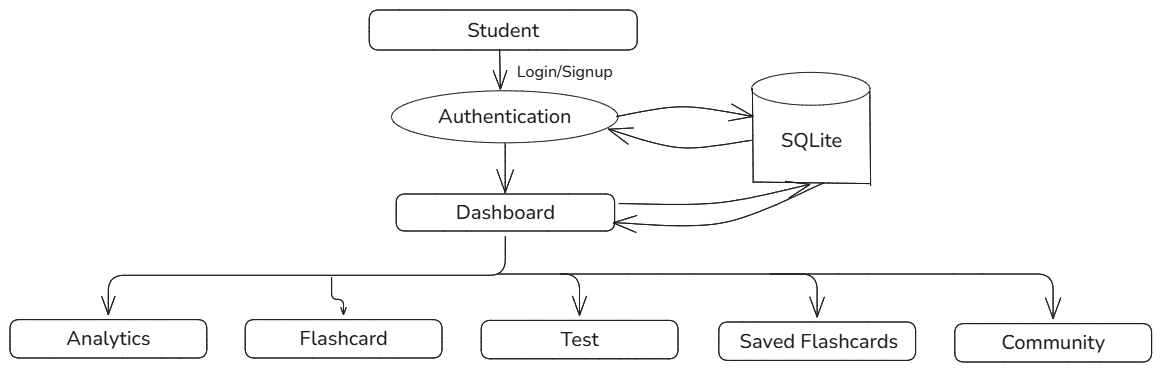
\includegraphics[width=\textwidth]{DFD 0.png}
    \caption{Level 0 DFD}
\end{figure}
\clearpage


\vspace{-\baselineskip} % Adjust vertical space here

\subsection{Level 1 DFD}
\Large
The Level 1 DFD expands on the Level 0 DFD by detailing the main processes identified previously, breaking them down into more specific sub-processes. It illustrates the interactions between these sub-processes and the data flows that connect them. \\

\begin{figure}[h]
    \centering
    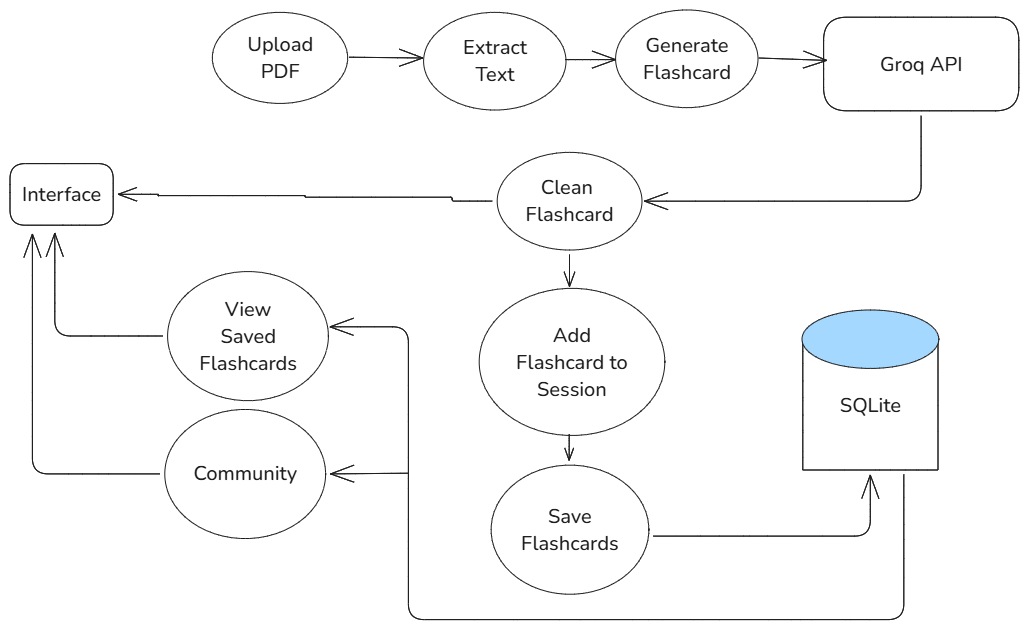
\includegraphics[width=\textwidth]{DFD level 1 part 1.png}
    \caption{Level 1 DFD Part 1}
\end{figure}
\begin{figure}[h]
    \centering
    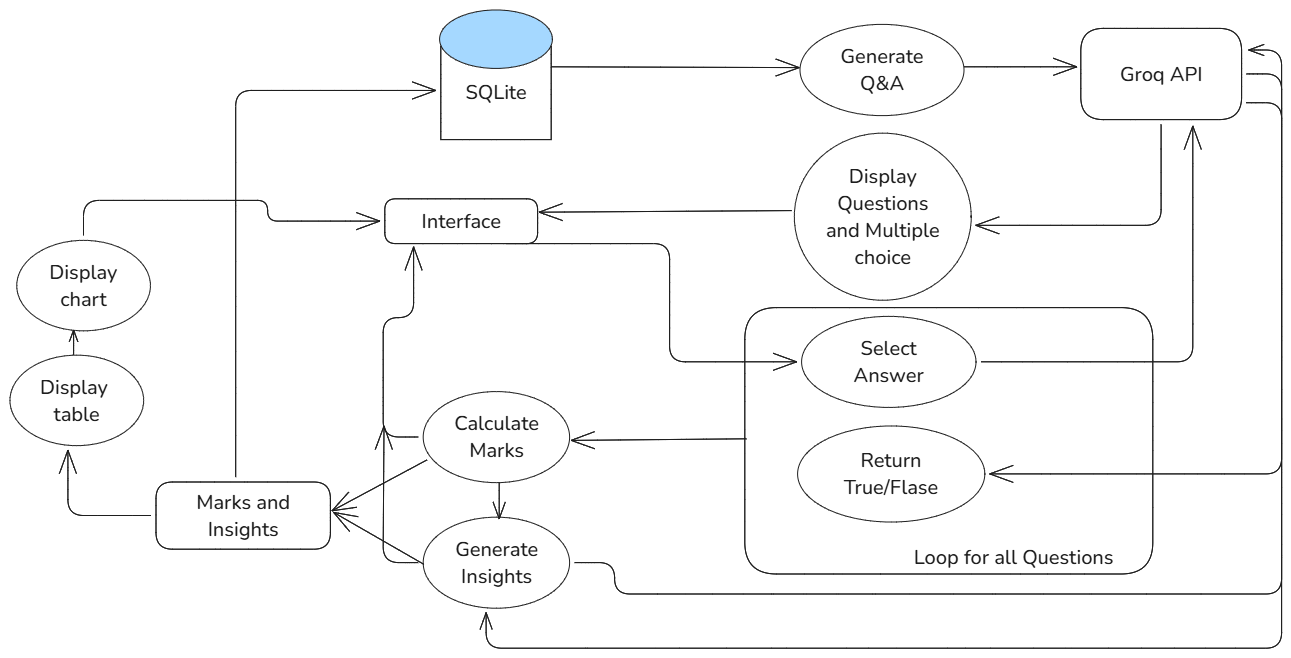
\includegraphics[width=\textwidth]{DFD level 1 part 2.png}
    \caption{Level 1 DFD Part 2}
\end{figure}
\clearpage

\vspace{-\baselineskip} % Adjust vertical space here

\subsection{Use Case Diagram}
\Large
The Use Case Diagram provides a visual representation of the interactions between users (students and educators) and the EduFlash system. It outlines the key functionalities and how different users will interact with the platform to enhance the learning experience. \\

\begin{figure}[h]
    \centering
    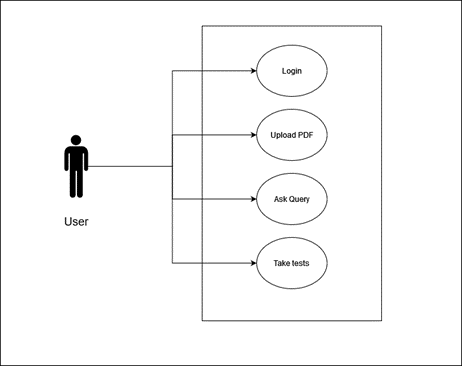
\includegraphics[width=\textwidth]{usecasediagram.png}
    \caption{Use Case Diagram}
\end{figure}

\section{Modular Design}

% Authentication Module
\subsection{Authentication Module}
The authentication module manages user access through secure login and signup processes.
\begin{figure}[H]
\centering
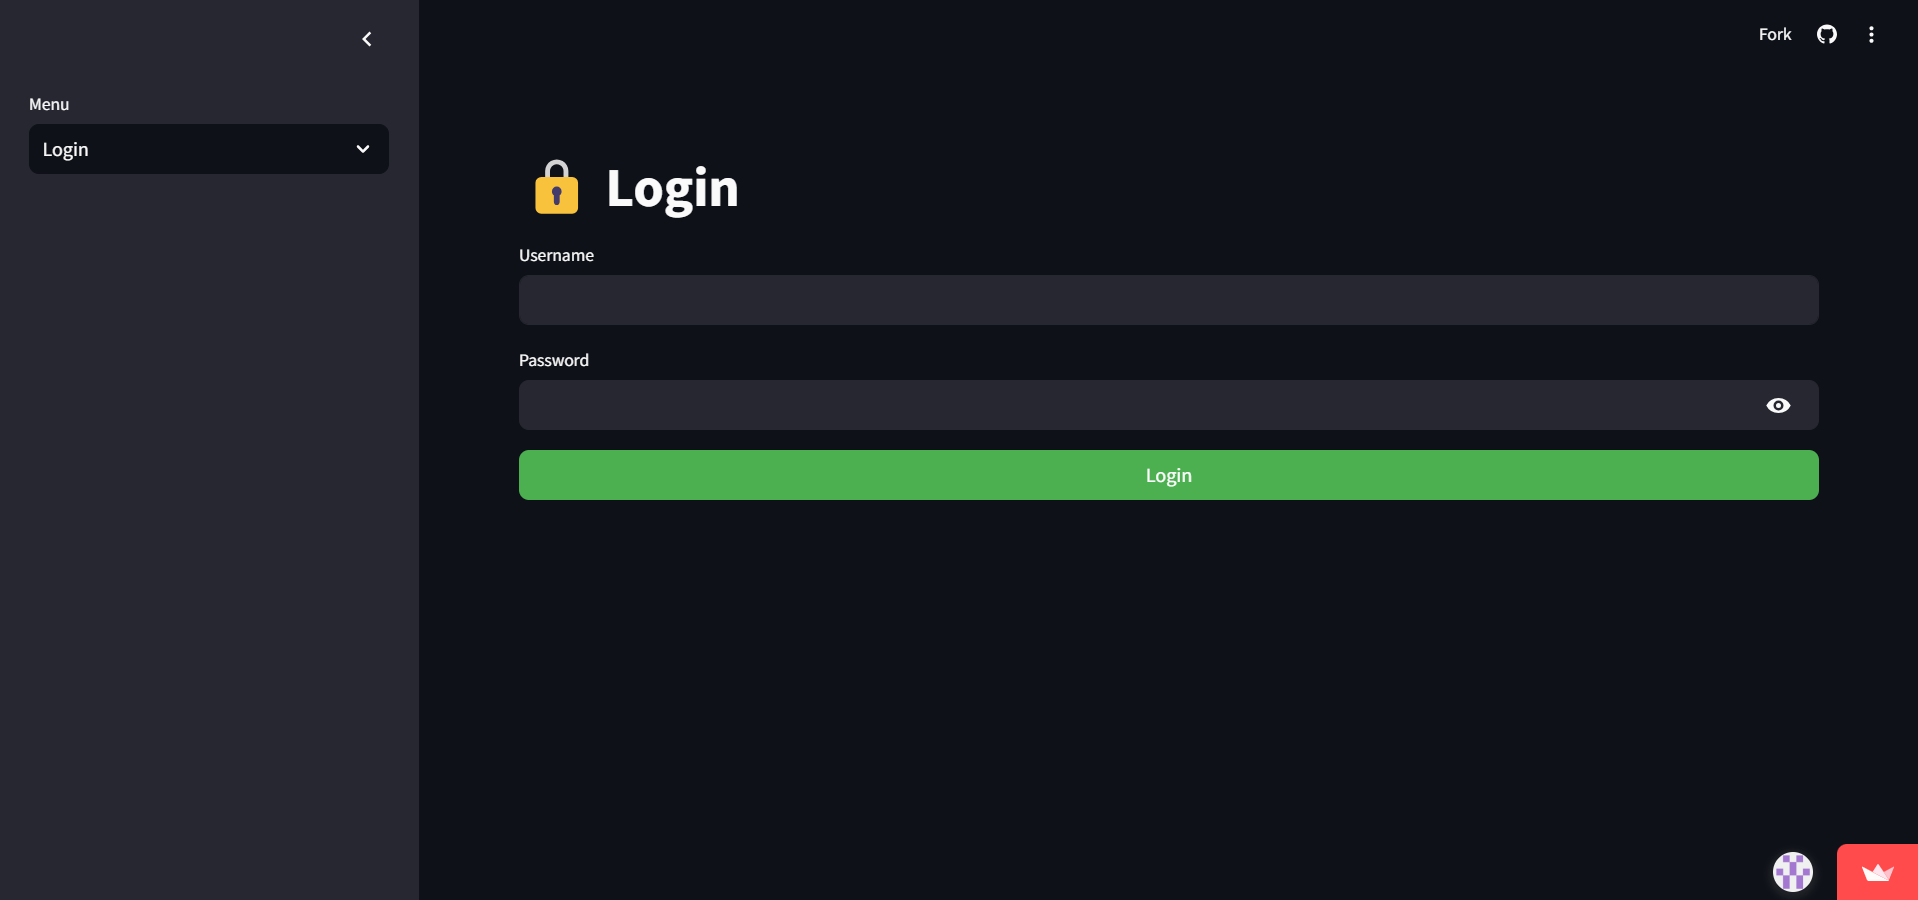
\includegraphics[width=0.9\textwidth]{login.png}
\caption{Login Screen}
\end{figure}
\begin{figure}[H]
\centering
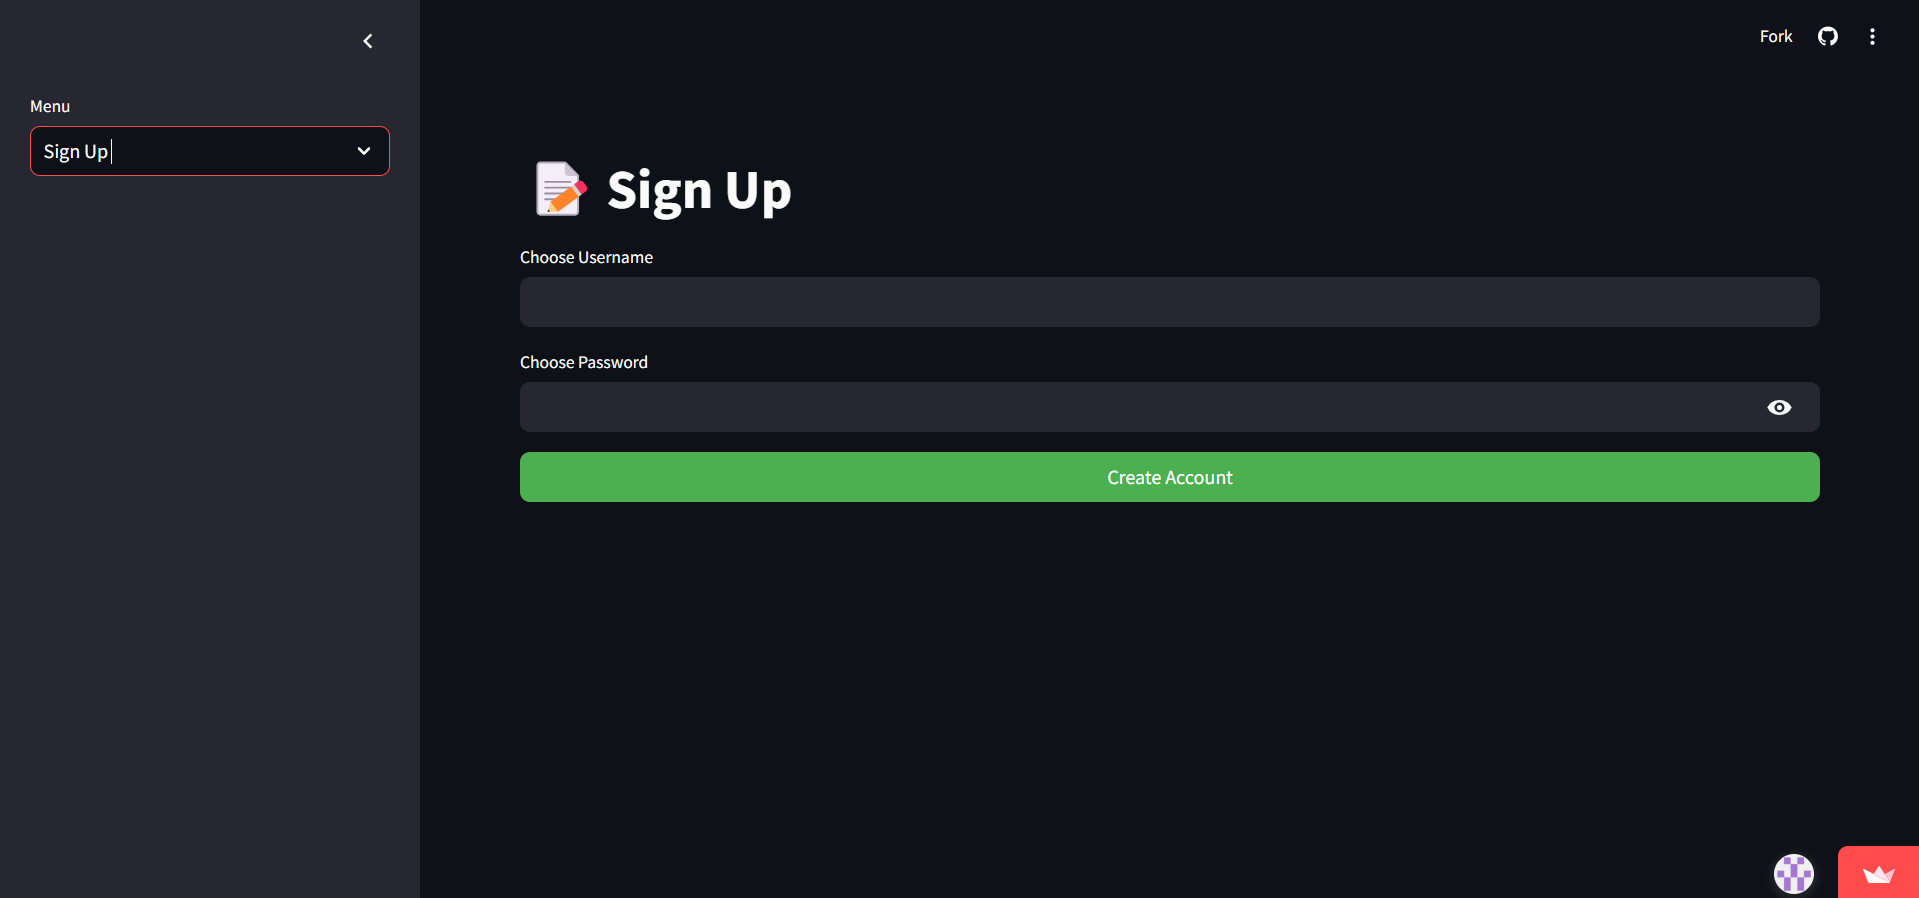
\includegraphics[width=0.9\textwidth]{signup.png}
\caption{Signup Screen}
\end{figure}
\begin{figure}[H]
\centering
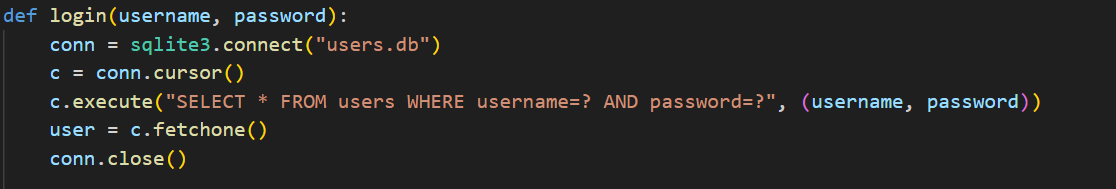
\includegraphics[width=0.9\textwidth]{login-code.png}
\caption{Login Code Snippet}
\end{figure}
\begin{figure}[H]
\centering
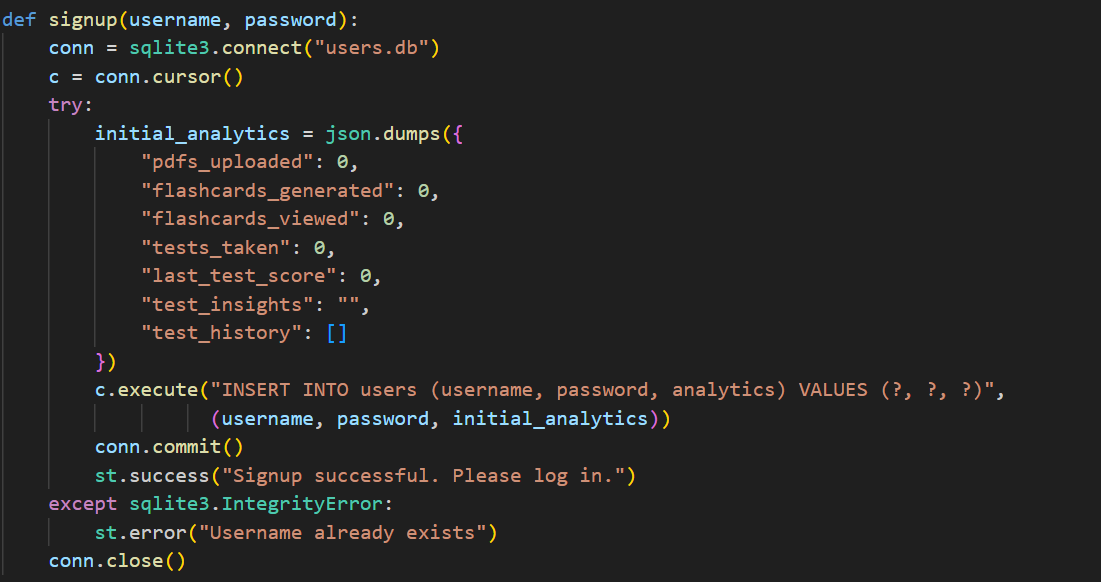
\includegraphics[width=0.9\textwidth]{signup-code.png}
\caption{Signup Code Snippet}
\end{figure}

% Dashboard
\subsection{Dashboard}
The dashboard provides an overview of user activities and progress.
\begin{figure}[H]
\centering
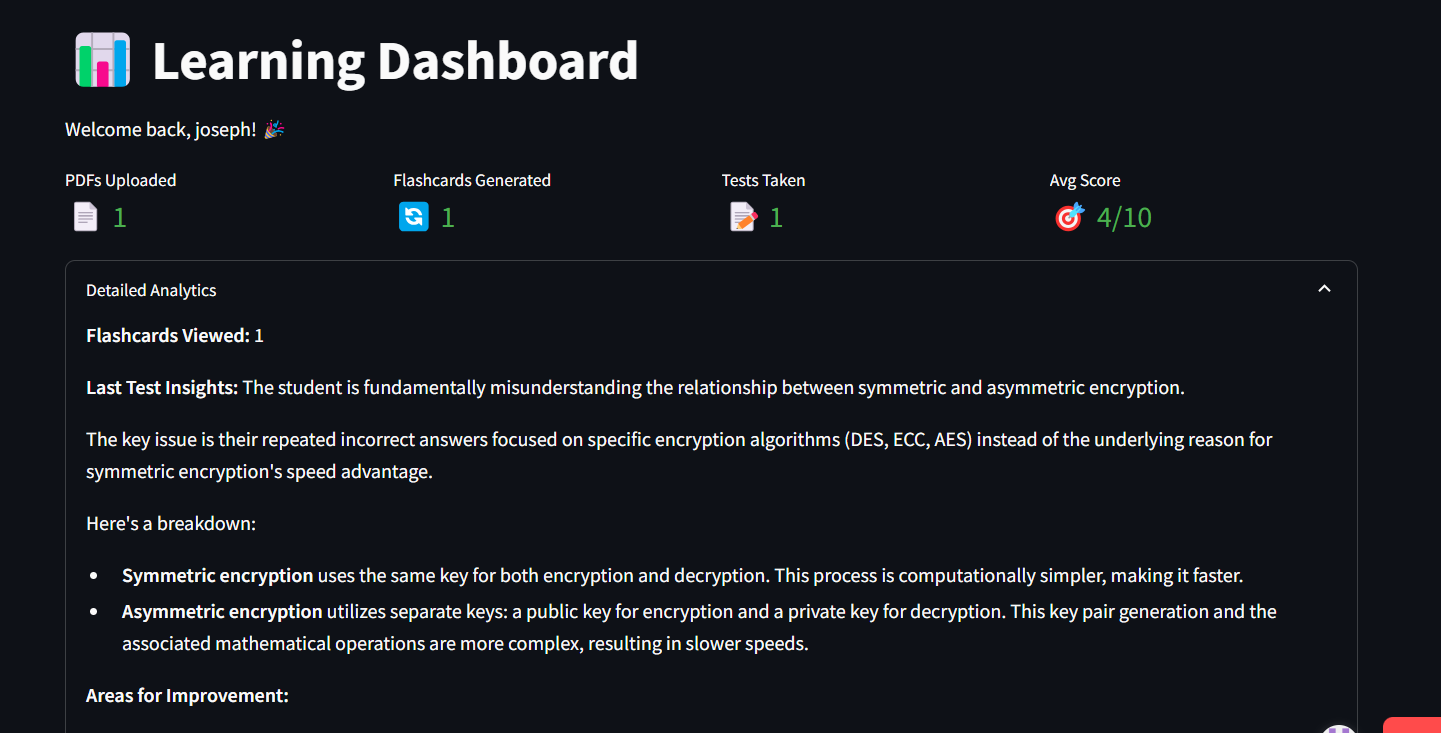
\includegraphics[width=0.9\textwidth]{dashboard.png}
\caption{User Dashboard}
\end{figure}
\begin{figure}[H]
\centering
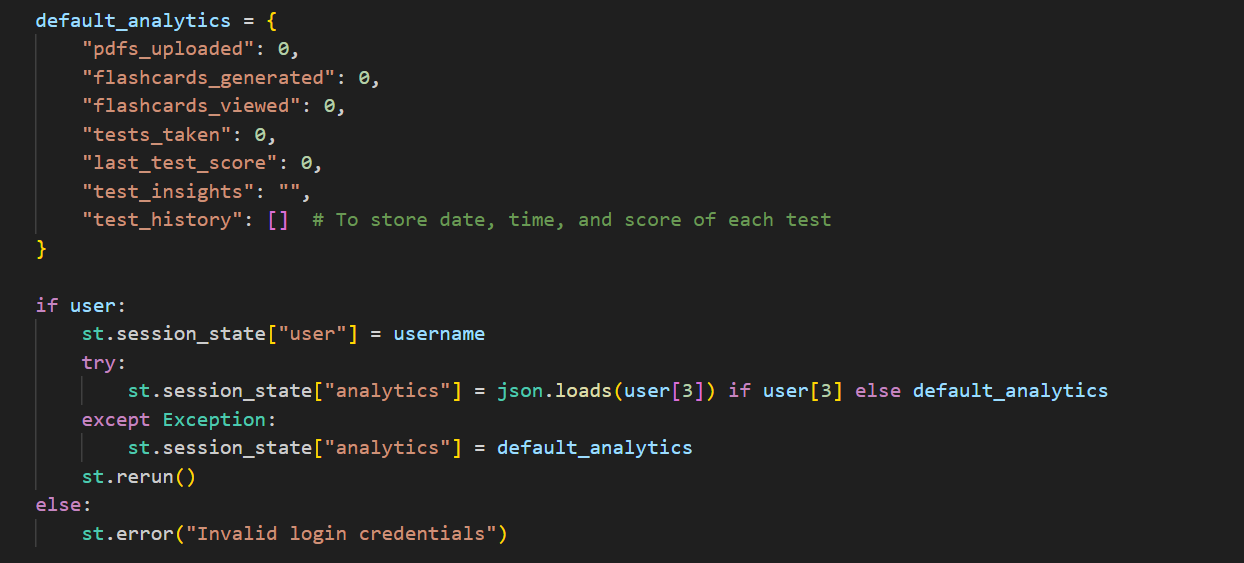
\includegraphics[width=0.9\textwidth]{dashboard-code.png}
\caption{Dashboard Code Snippet}
\end{figure}

% Flashcard Session
\subsection{Flashcard Session}
This module facilitates interactive learning through flashcards.
\begin{figure}[H]
\centering
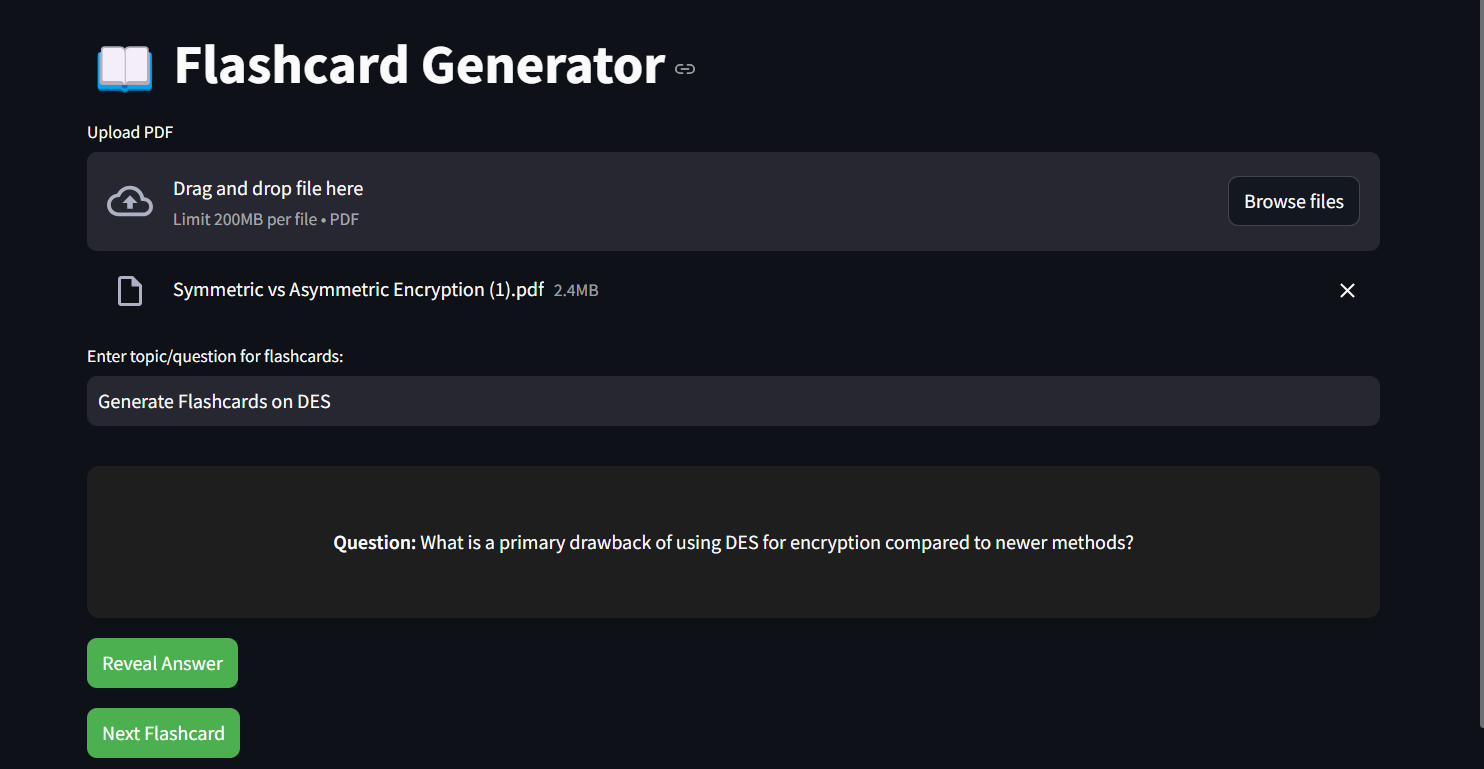
\includegraphics[width=0.9\textwidth]{flashcard-question.png}
\caption{Flashcard Session - Question}
\end{figure}
\begin{figure}[H]
\centering
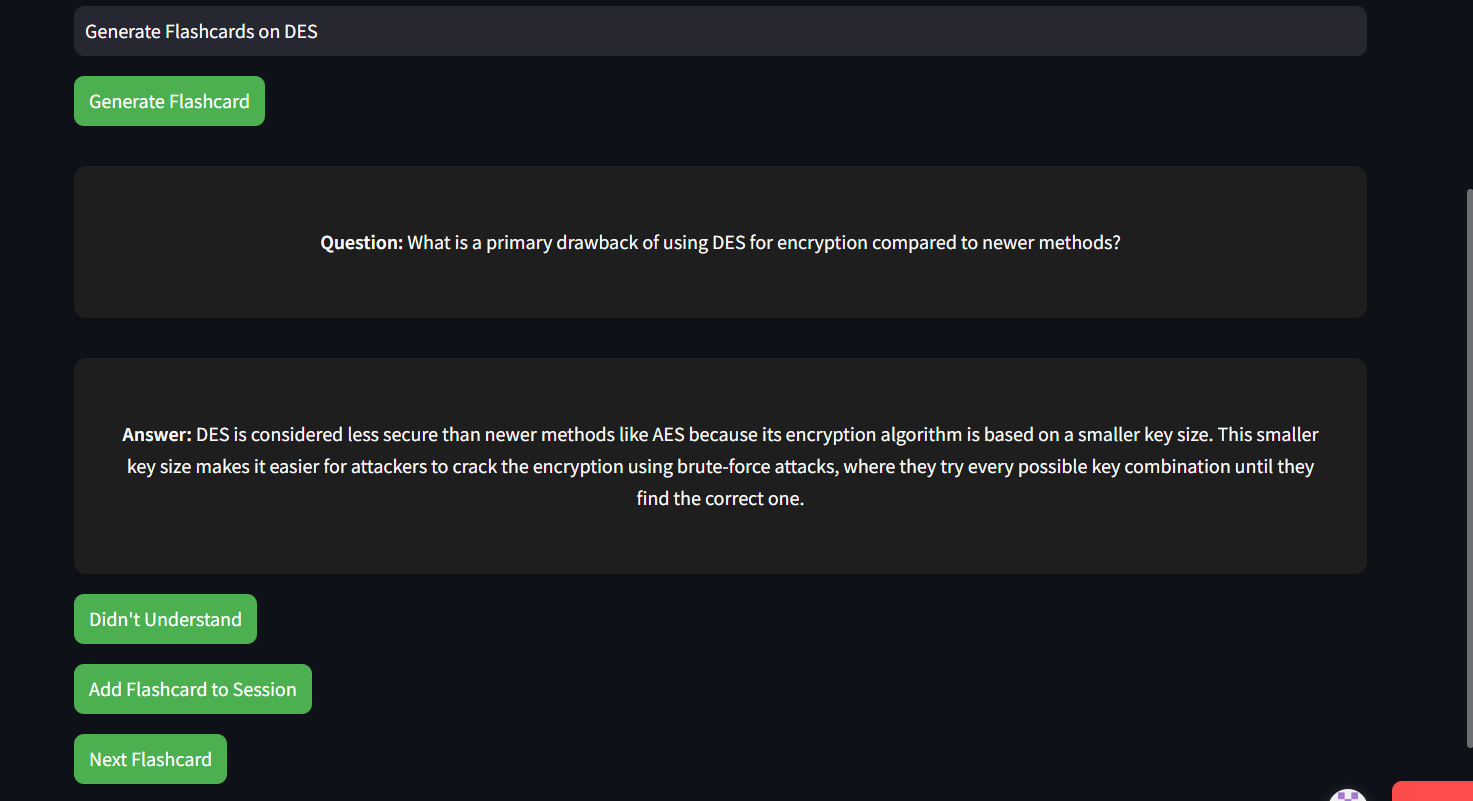
\includegraphics[width=0.9\textwidth]{flashcard-answer.png}
\caption{Flashcard Session - Answer}
\end{figure}
\begin{figure}[H]
\centering
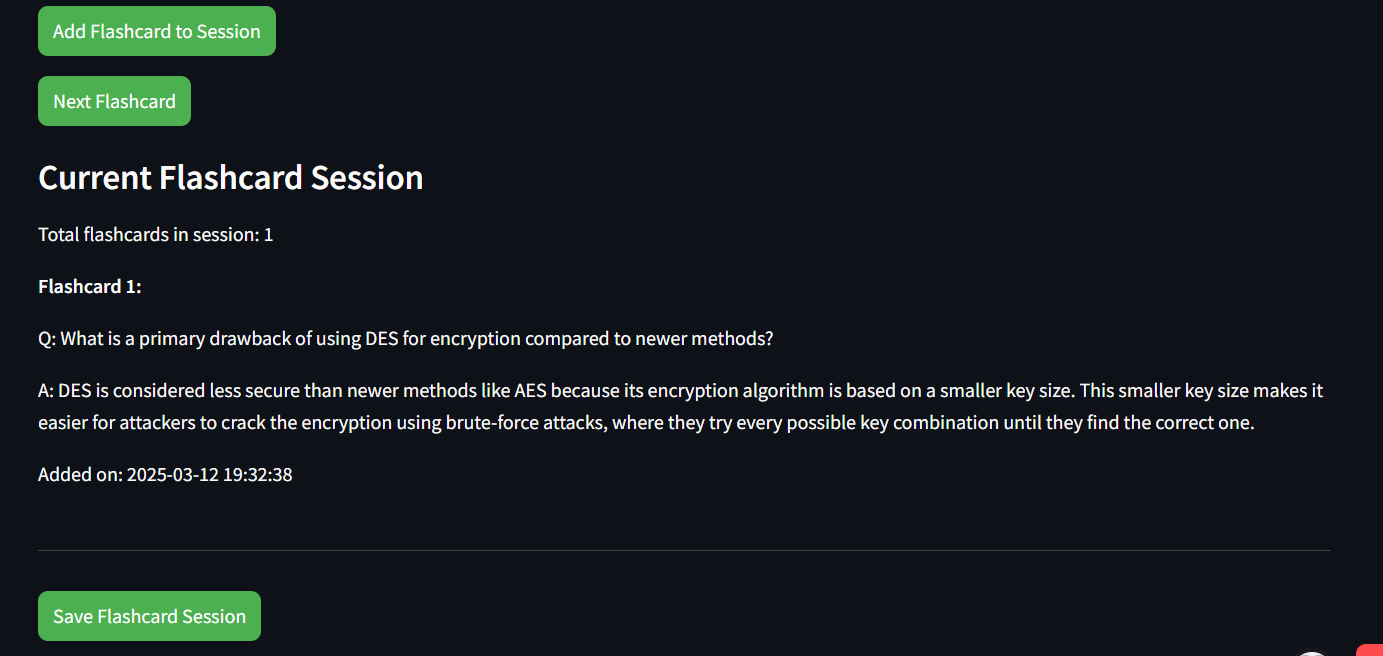
\includegraphics[width=0.9\textwidth]{saving-flashcard.png}
\caption{Flashcard Session - Saving}
\end{figure}
\begin{figure}[H]
\centering
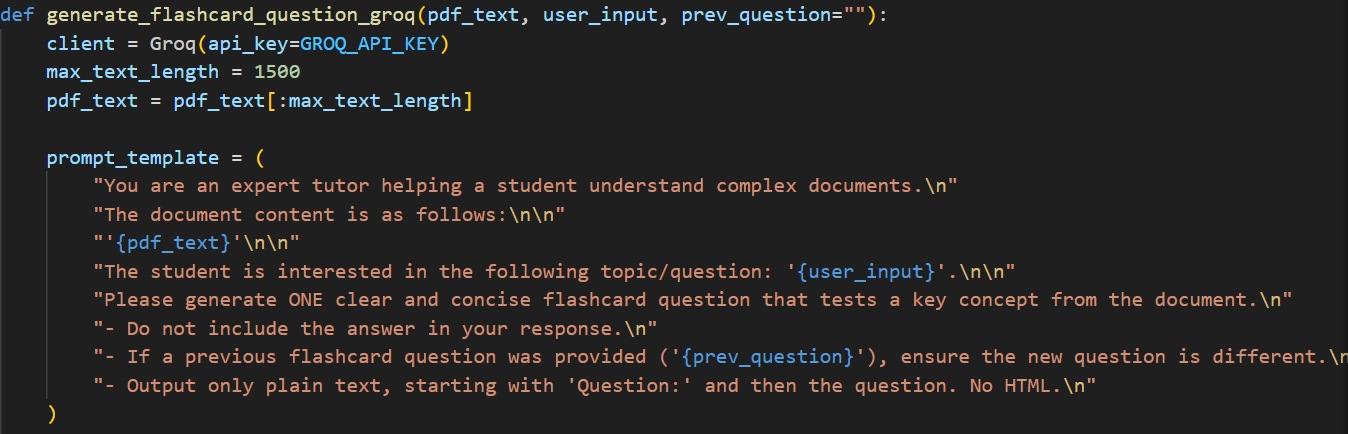
\includegraphics[width=0.9\textwidth]{flashcard-groq-code.png}
\caption{Flashcard Question Code Snippet}
\end{figure}
\begin{figure}[H]
\centering
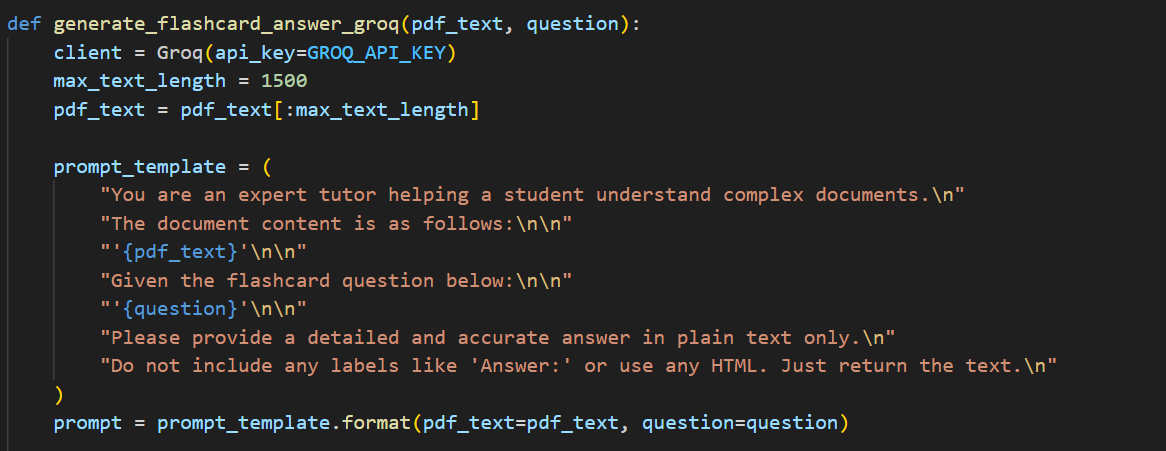
\includegraphics[width=0.9\textwidth]{flashcard-ans-groq-code.png}
\caption{Flashcard Answer Code Snippet}
\end{figure}
\begin{figure}[H]
\centering
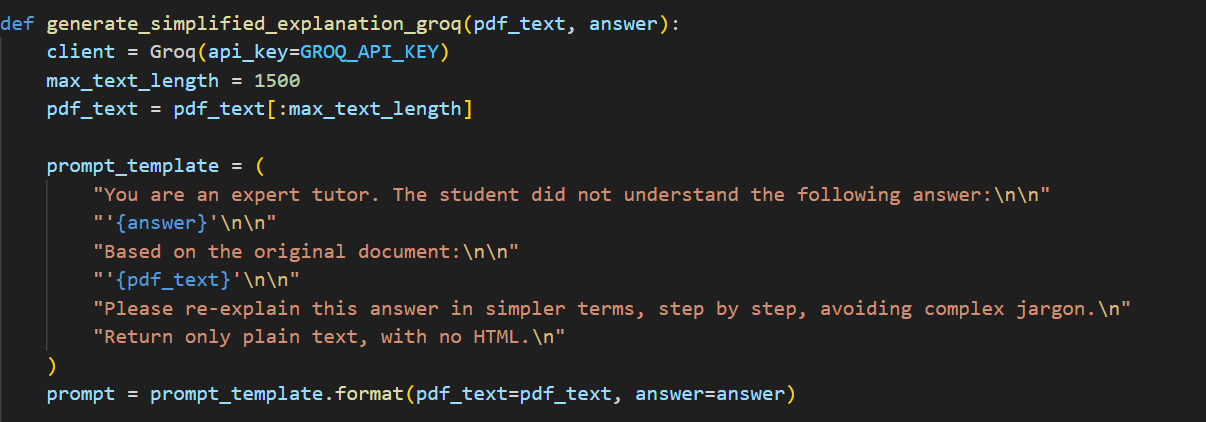
\includegraphics[width=0.9\textwidth]{simple-exp-code.png}
\caption{Flashcard Explanation Code Snippet}
\end{figure}

% Saved Flashcard Session
\subsection{Saved Flashcard Session}
Allows users to revisit previously saved flashcards.
\begin{figure}[H]
\centering
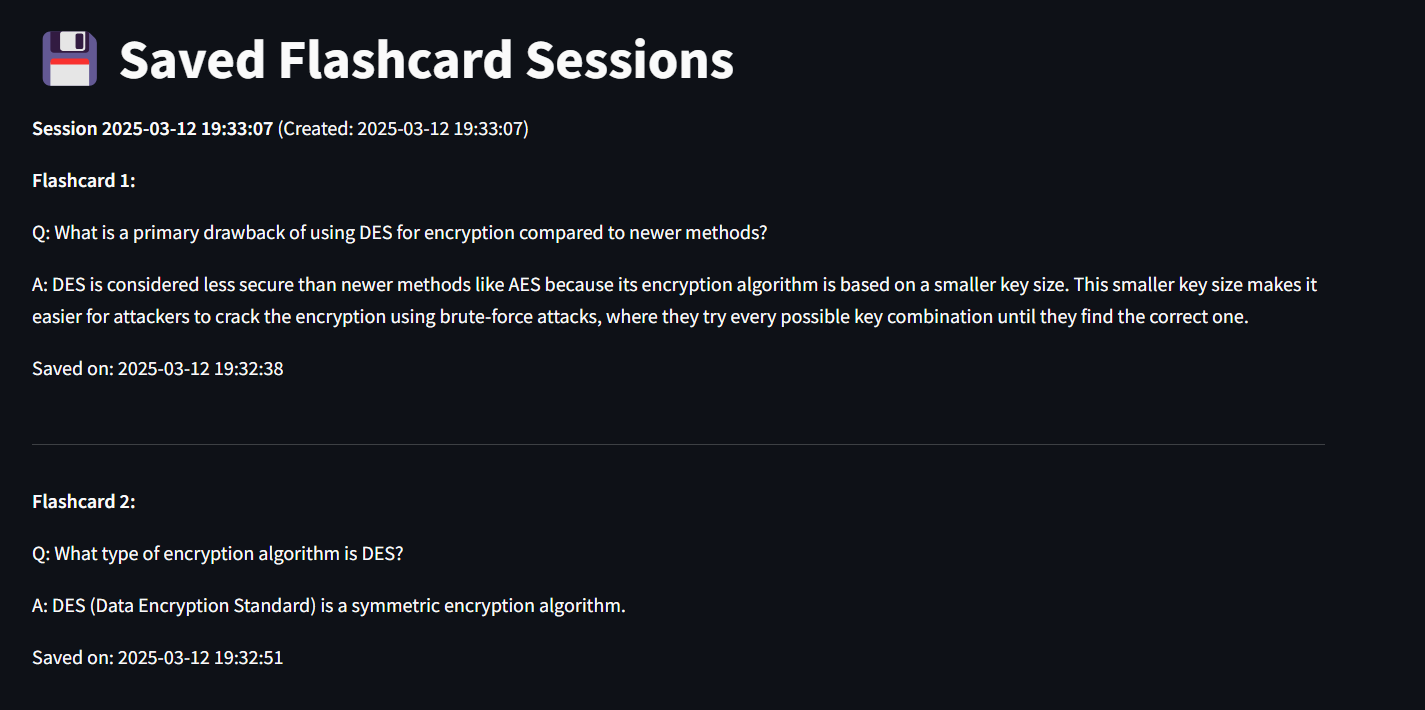
\includegraphics[width=0.9\textwidth]{saved-flashcard.png}
\caption{Saved Flashcards}
\end{figure}

% Test Session
\subsection{Test Session}
Engages users in quizzes and tests to reinforce learning.
\begin{figure}[H]
\centering
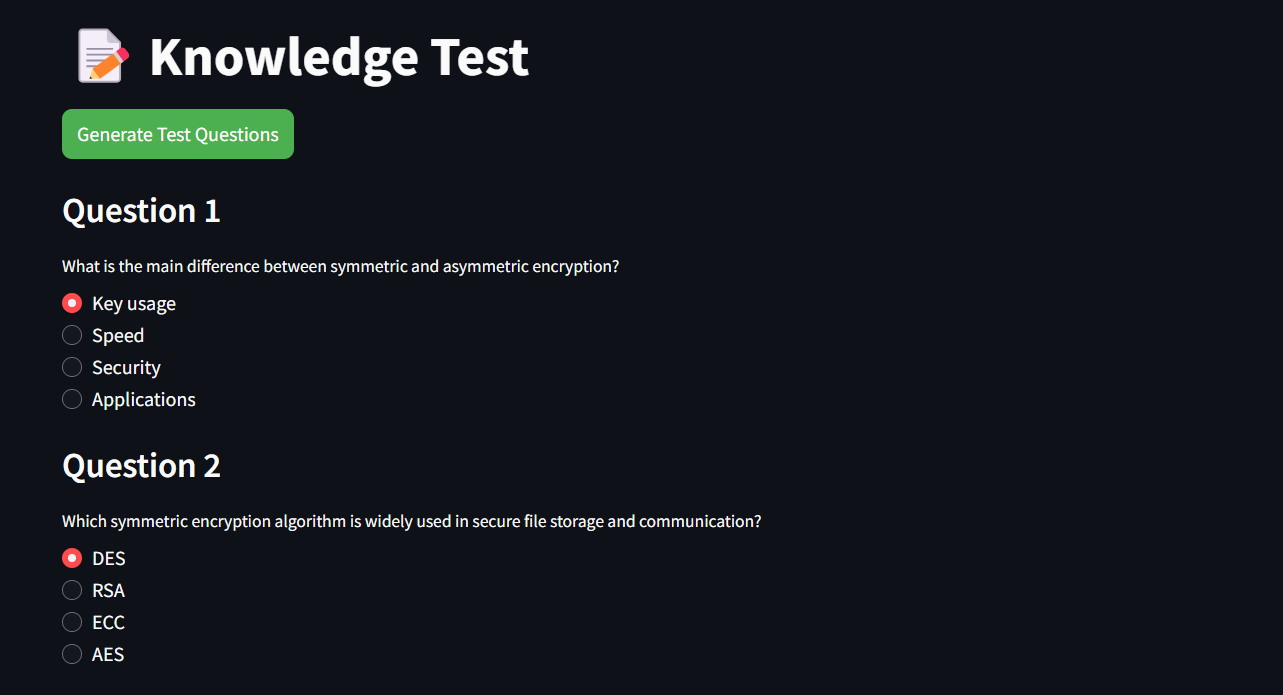
\includegraphics[width=0.9\textwidth]{test.png}
\caption{Test Session - Question}
\end{figure}
\begin{figure}[H]
\centering
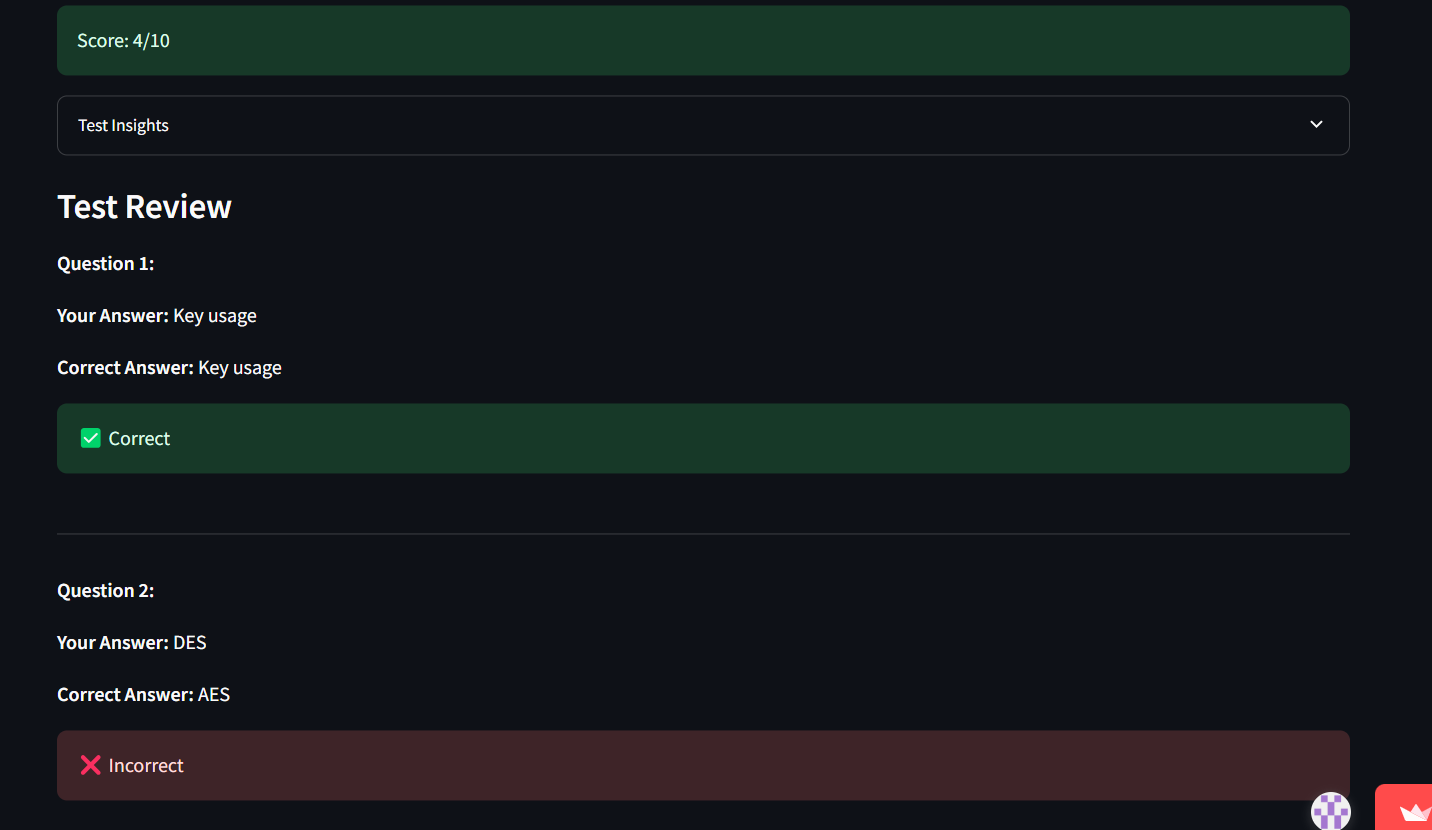
\includegraphics[width=0.9\textwidth]{test-score-result.png}
\caption{Test Session - Results}
\end{figure}
\begin{figure}[H]
\centering
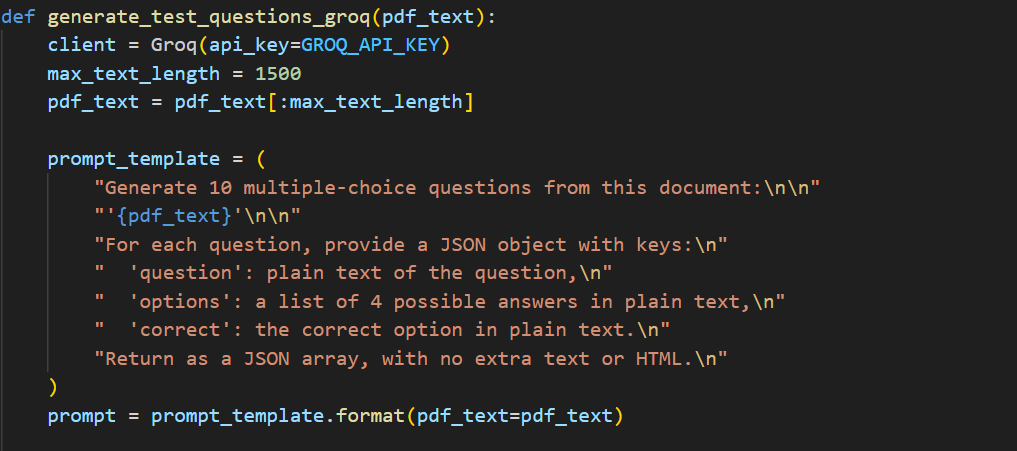
\includegraphics[width=0.9\textwidth]{test-code.png}
\caption{Test Code Snippet}
\end{figure}

% Community
\subsection{Community}
Facilitates interaction and collaboration among users.
\begin{figure}[H]
\centering
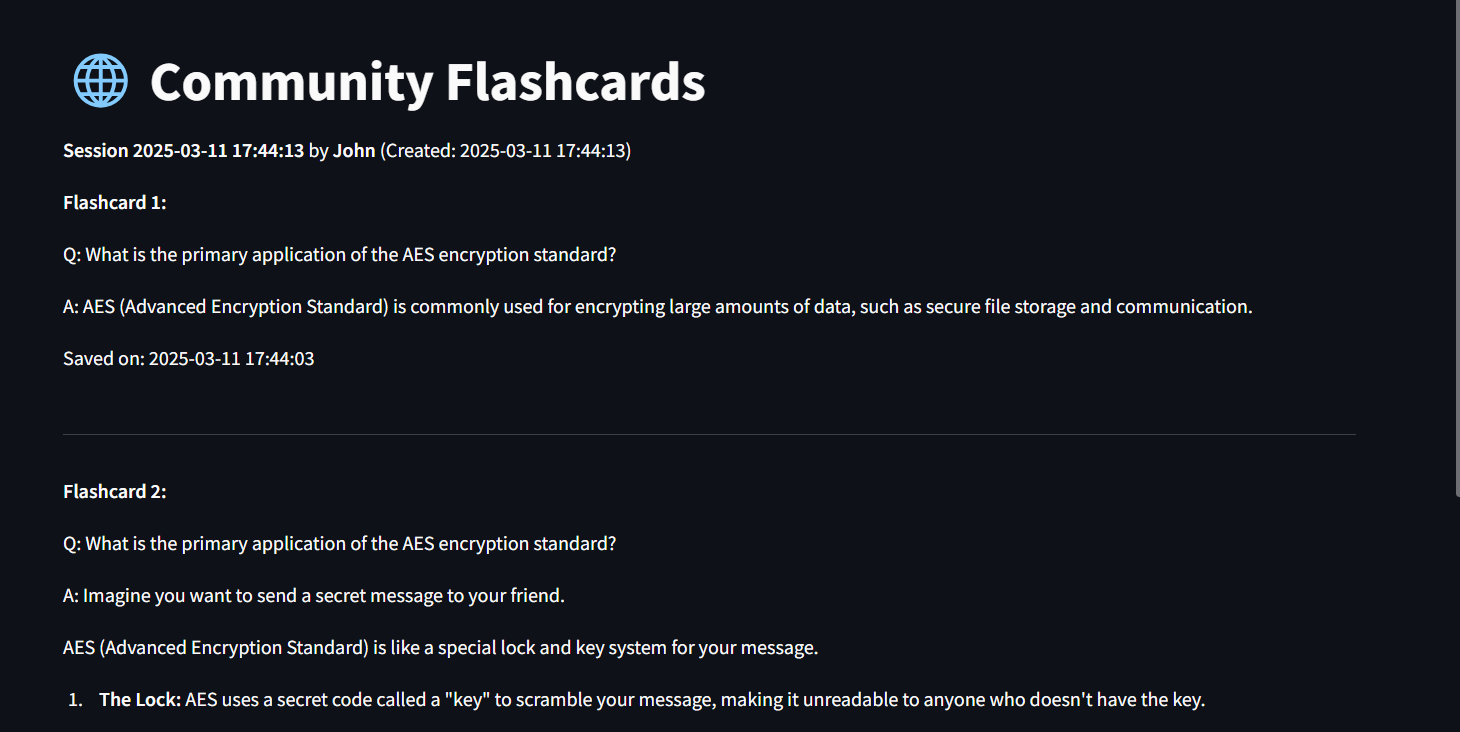
\includegraphics[width=0.9\textwidth]{community.png}
\caption{Community Features}
\end{figure}

% Test Insights
\subsection{Test Insights}
Provides detailed analytics and insights on user performance.
\begin{figure}[H]
\centering
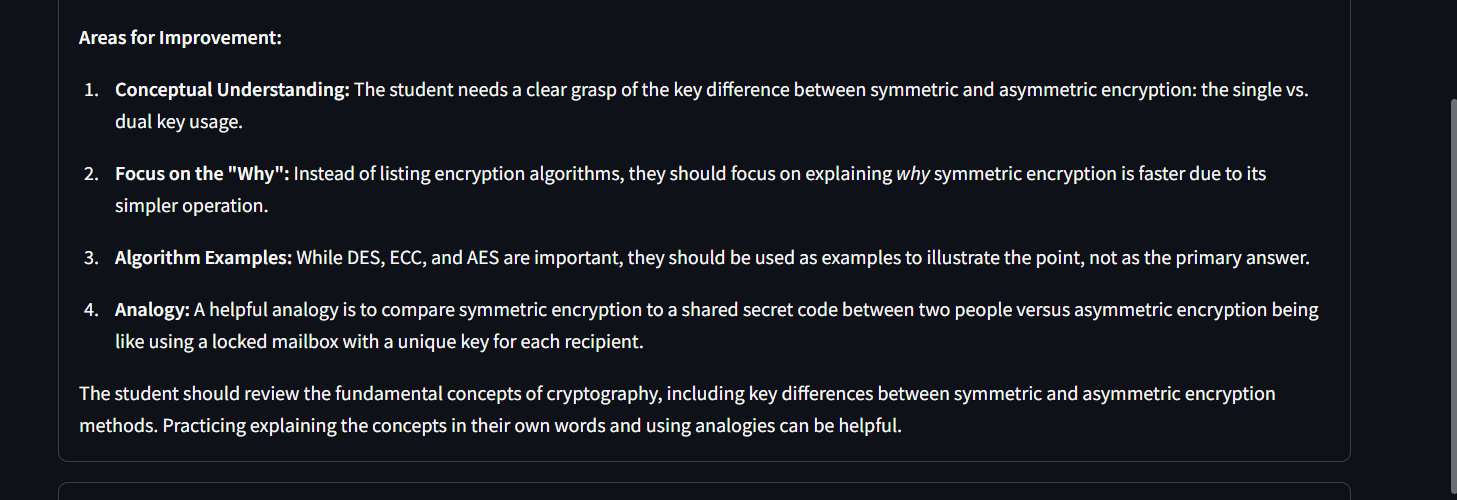
\includegraphics[width=0.9\textwidth]{test-insights.png}
\caption{Test Insights}
\end{figure}
\begin{figure}[H]
\centering
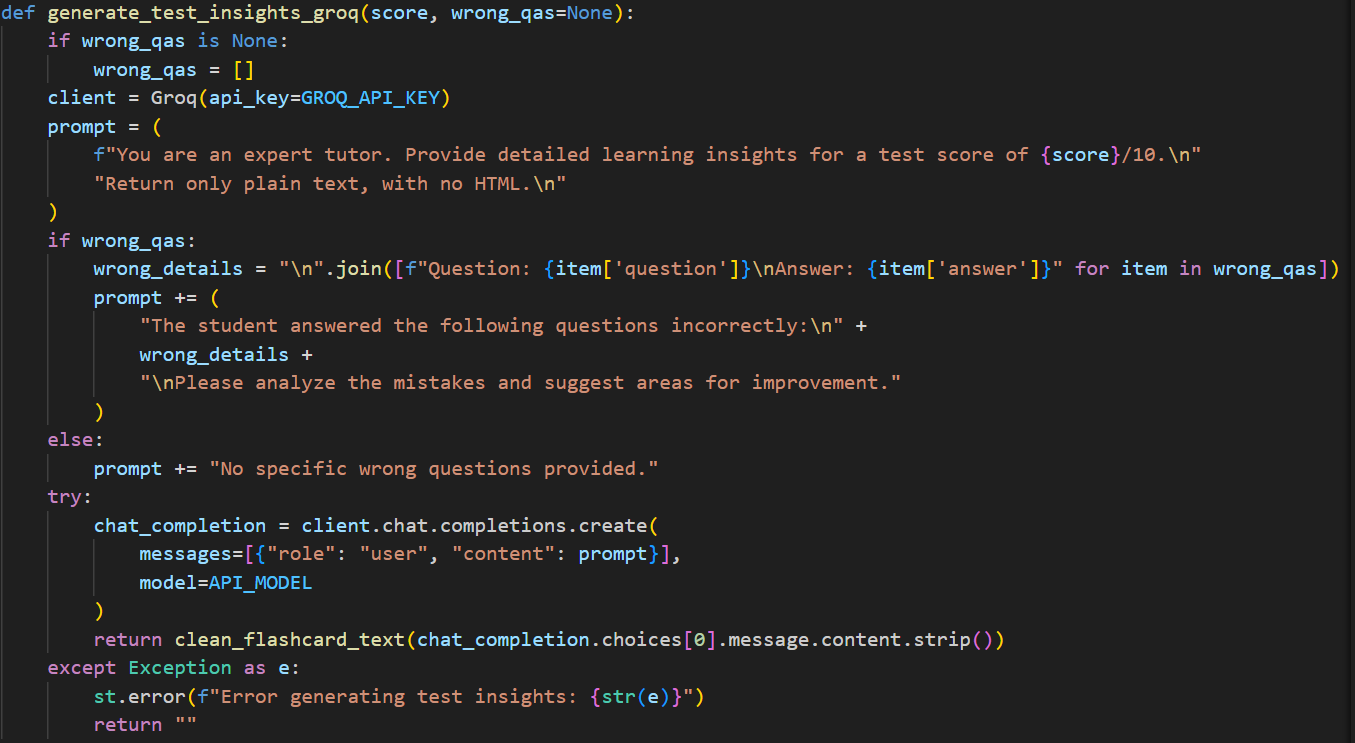
\includegraphics[width=0.9\textwidth]{test-insights-code.png}
\caption{Test Insights Code Snippet}
\end{figure}

% Graph and Table Section
\subsection{Graph and Table Section}
Displays data visualizations to track progress and performance.
\begin{figure}[H]
\centering
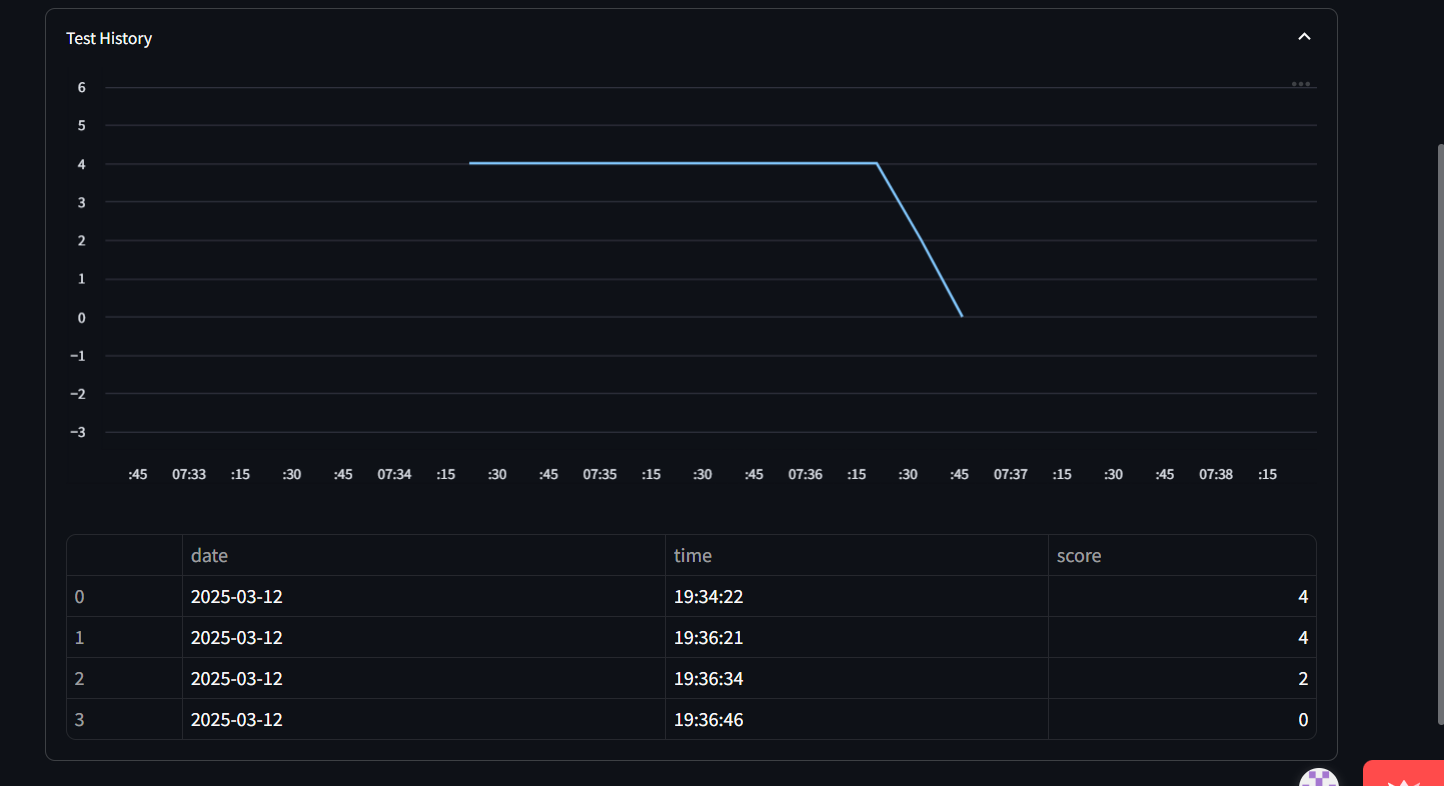
\includegraphics[width=0.9\textwidth]{graph-table.png}
\caption{Graphs and Tables}
\end{figure}
\begin{figure}[H]
\centering
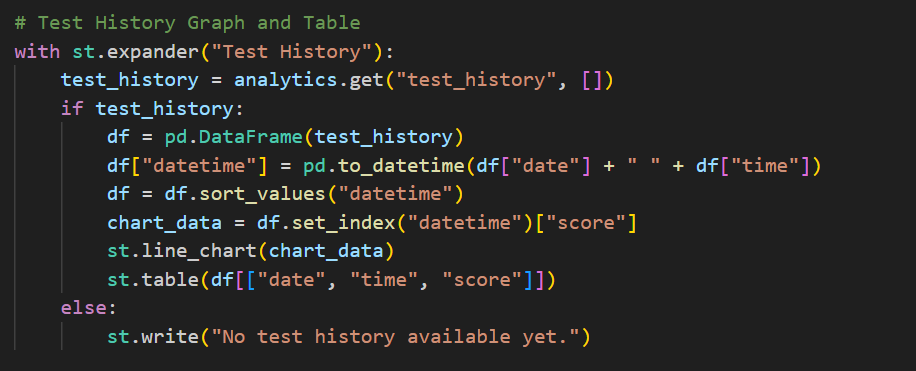
\includegraphics[width=0.9\textwidth]{graph-table-code.png}
\caption{Graph and Table Code Snippet}
\end{figure}
\clearpage
\FloatBarrier % Ensure all floats are processed before moving to the next section

\section{Modules Used}
The EduFlash platform is designed with several key modules to ensure a seamless and effective learning experience:
\begin{itemize}
    \item \textbf{User Authentication:} Managed using Auth0, providing secure login and role-based access.
    \item \textbf{PDF Processing:} Utilizes PyPDF2 for extracting text from uploaded PDFs, which is then analyzed for flashcard generation.
    \item \textbf{Flashcard Generation:} Employs AI algorithms via the Groq API to create personalized flashcards based on extracted content.
    \item \textbf{Real-Time Feedback:} Implements interactive elements to assess student understanding and adapt teaching strategies accordingly.
    \item \textbf{Data Management:} Uses SQLite for efficient storage and retrieval of user data, flashcards, and progress tracking.
\end{itemize}

\chapter{System Implementation}
\section{Overview}
The system implementation of EduFlash involves both frontend and backend components, integrated to provide a cohesive user experience. The frontend is developed using Streamlit, offering an interactive and responsive interface, while the backend handles data processing and storage.

\section{Modular Design}

% Authentication Module
\subsection{Authentication Module}
The authentication module manages user access through secure login and signup processes.
\begin{figure}[H]
\centering
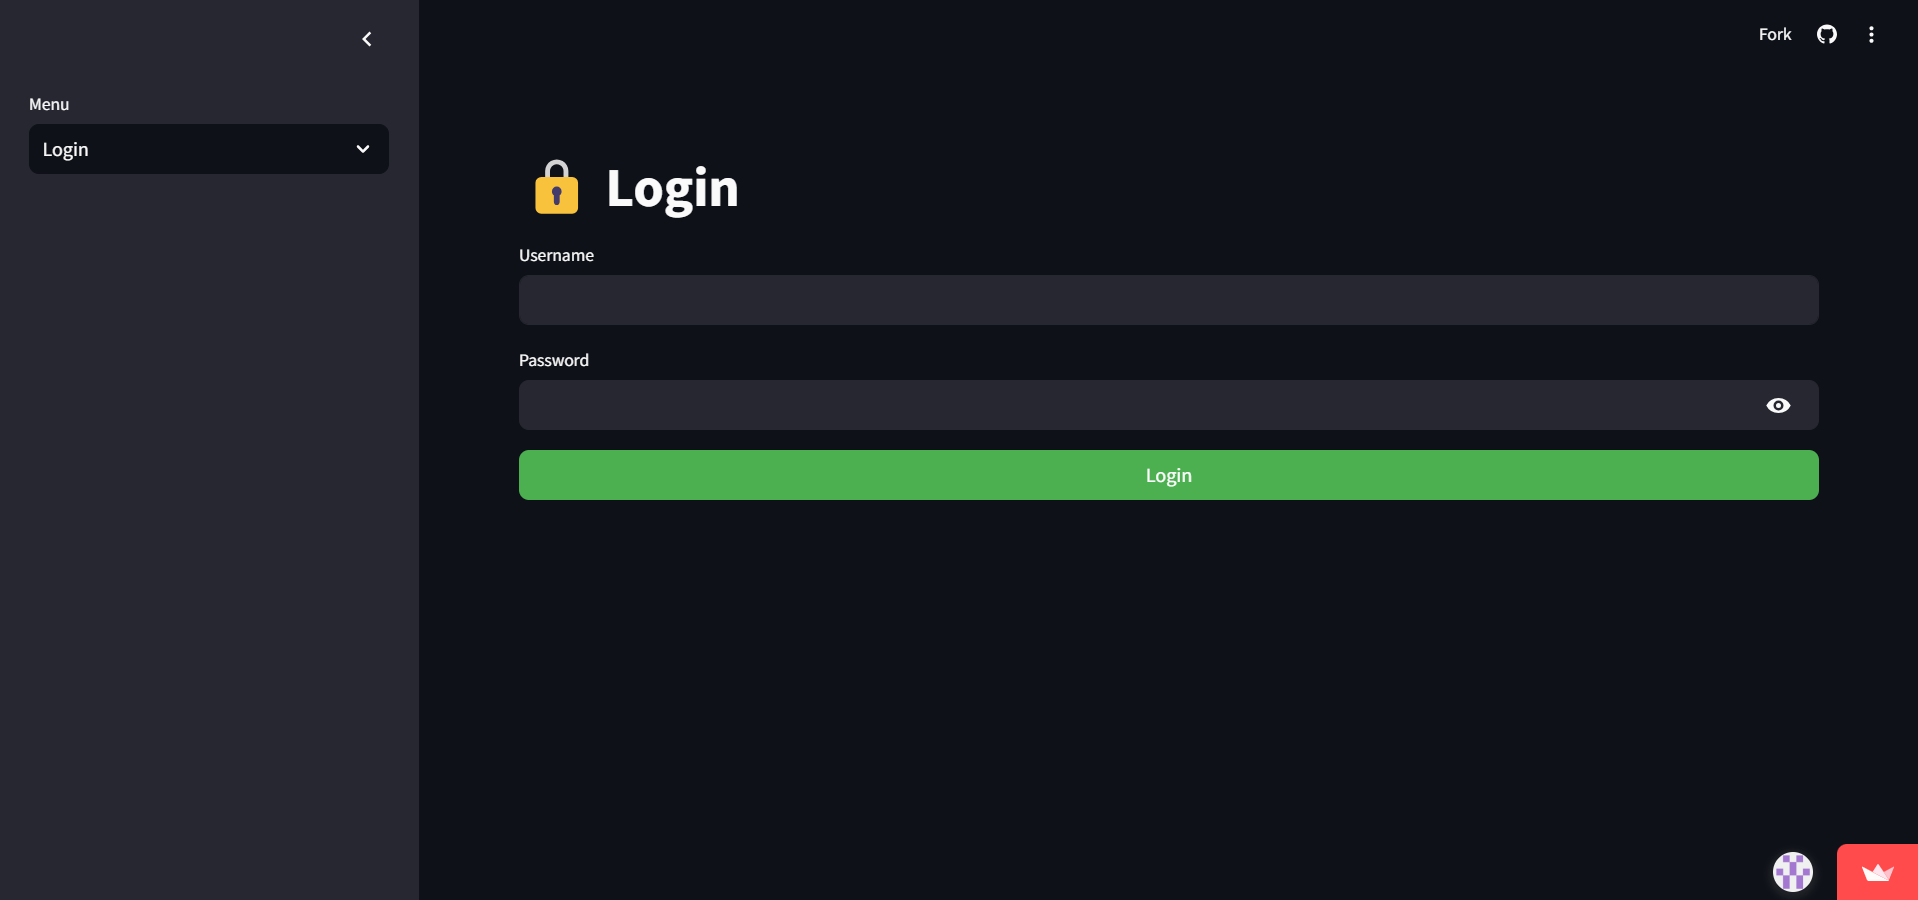
\includegraphics[width=0.9\textwidth]{login.png}
\caption{Login Screen}
\end{figure}
\begin{figure}[H]
\centering
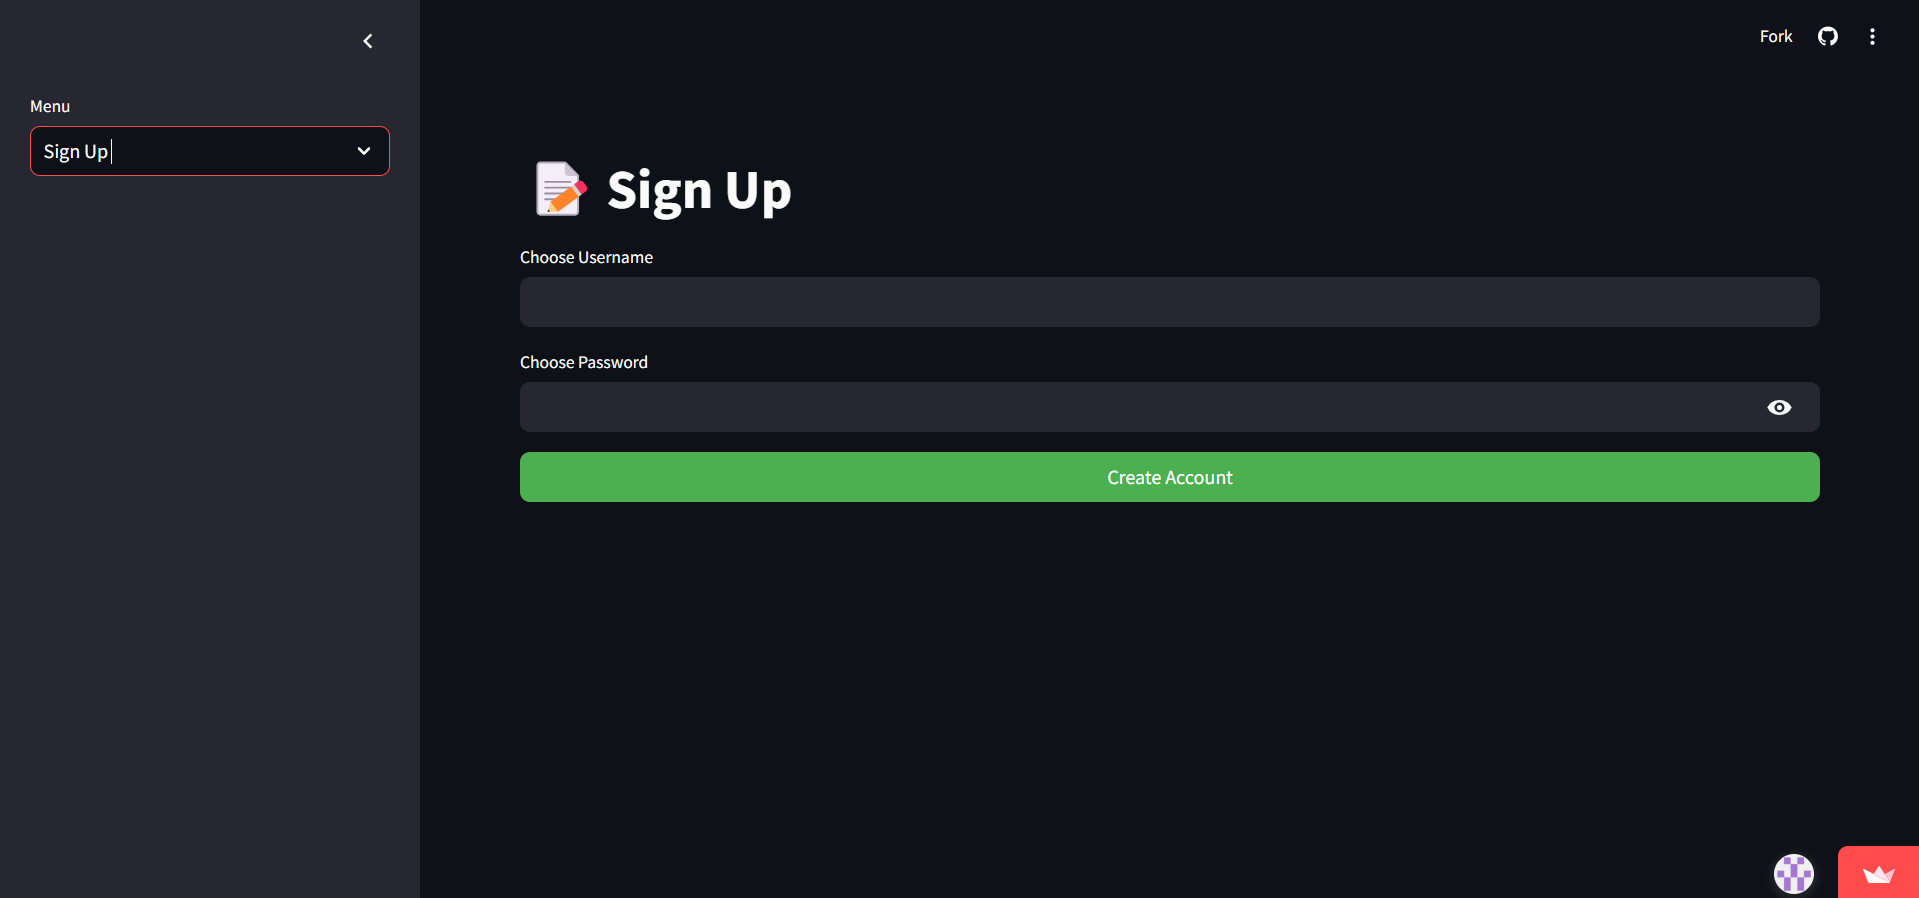
\includegraphics[width=0.9\textwidth]{signup.png}
\caption{Signup Screen}
\end{figure}
\begin{figure}[H]
\centering
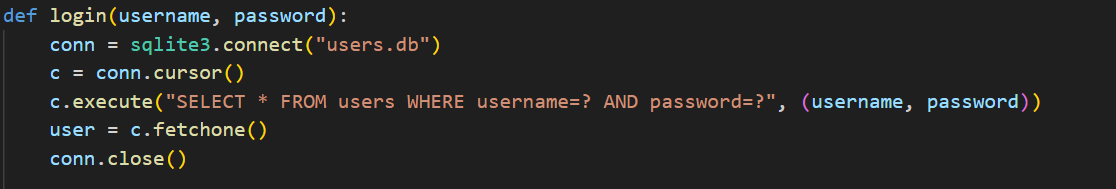
\includegraphics[width=0.9\textwidth]{login-code.png}
\caption{Login Code Snippet}
\end{figure}
\begin{figure}[H]
\centering
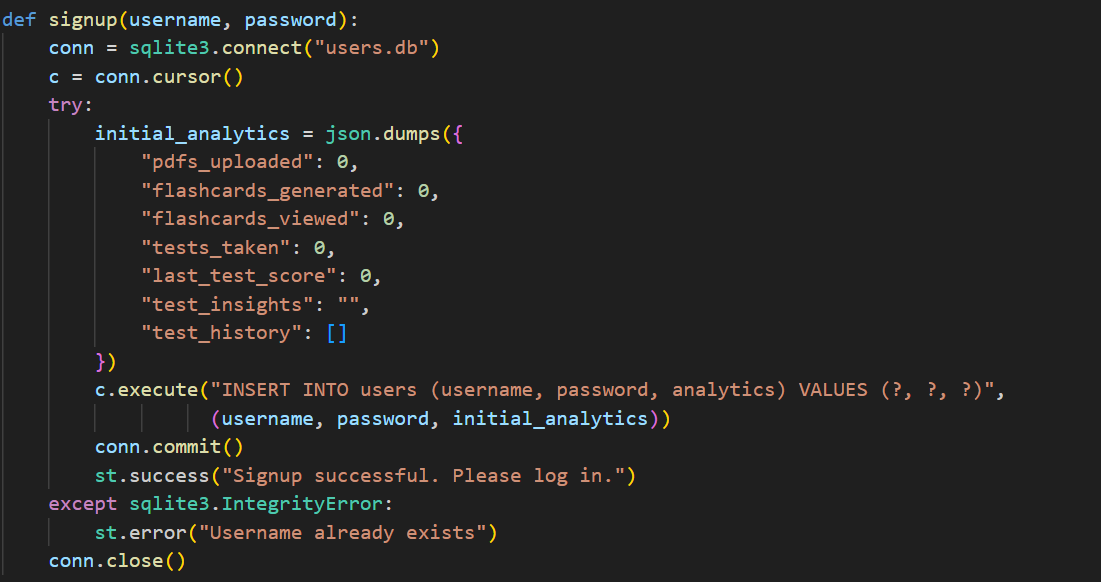
\includegraphics[width=0.9\textwidth]{signup-code.png}
\caption{Signup Code Snippet}
\end{figure}

% Dashboard
\subsection{Dashboard}
The dashboard provides an overview of user activities and progress.
\begin{figure}[H]
\centering
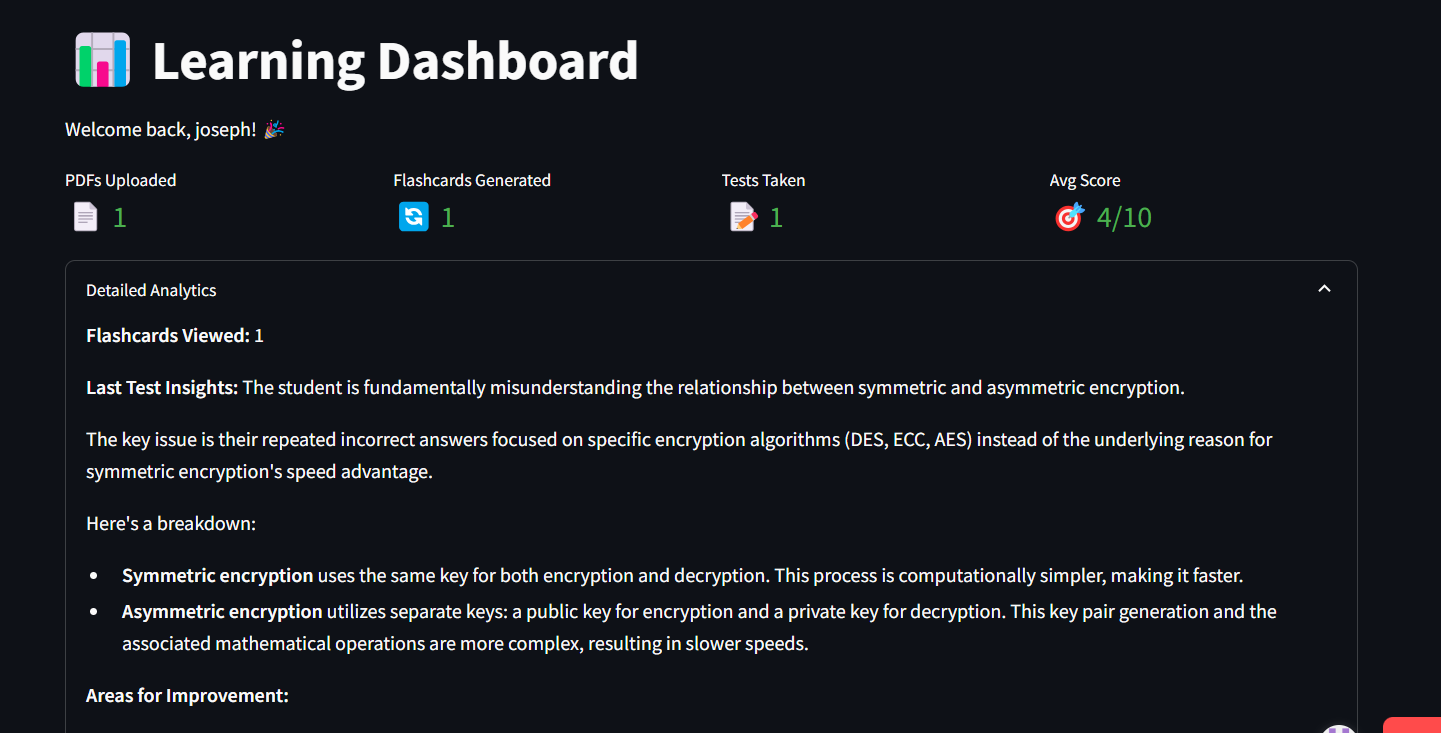
\includegraphics[width=0.9\textwidth]{dashboard.png}
\caption{User Dashboard}
\end{figure}
\begin{figure}[H]
\centering
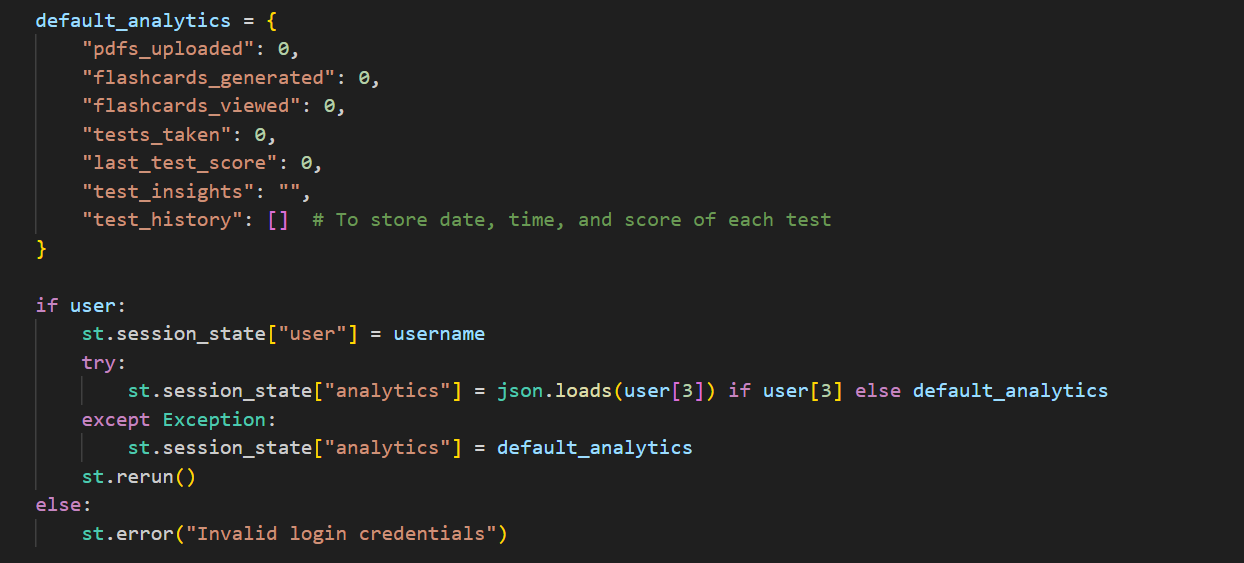
\includegraphics[width=0.9\textwidth]{dashboard-code.png}
\caption{Dashboard Code Snippet}
\end{figure}

% Flashcard Session
\subsection{Flashcard Session}
This module facilitates interactive learning through flashcards.
\begin{figure}[H]
\centering
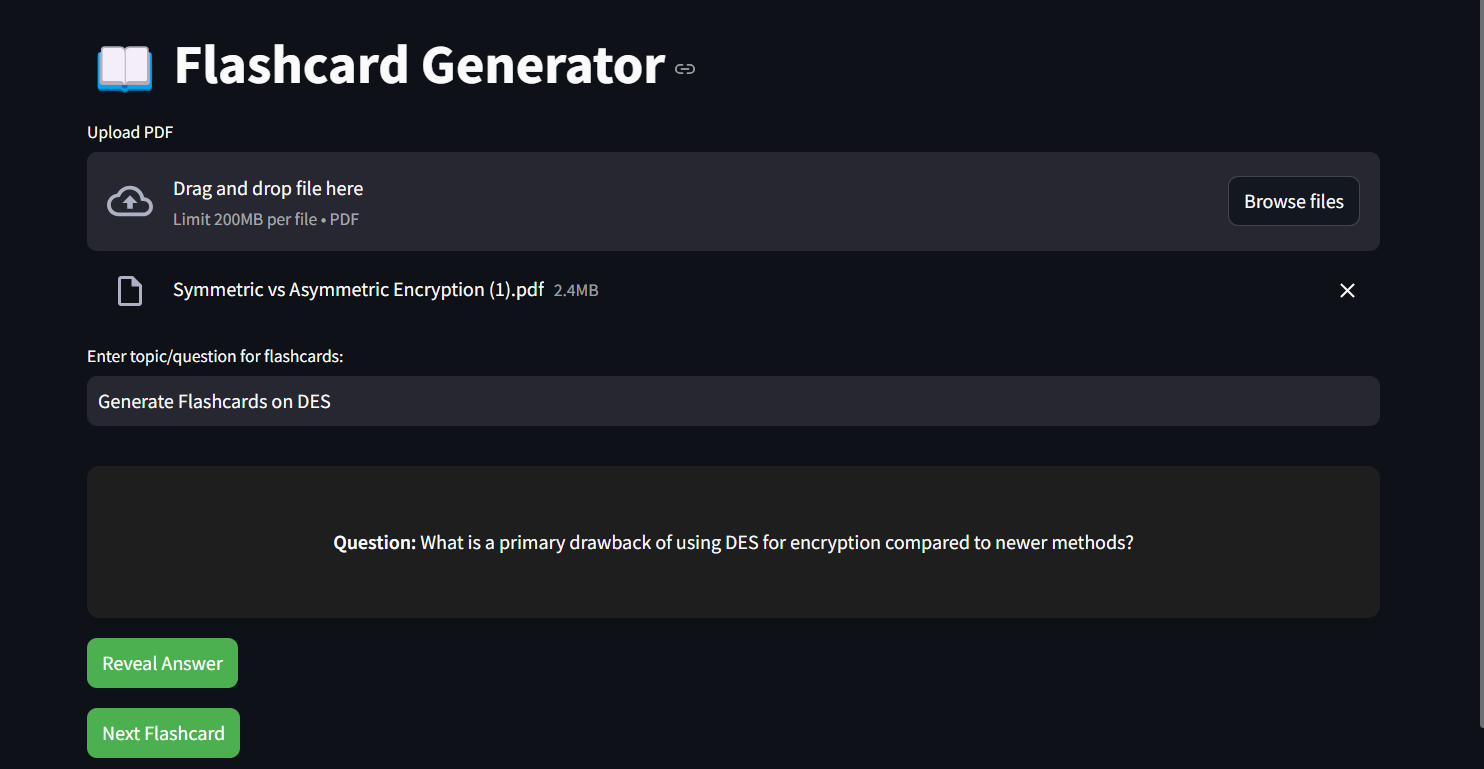
\includegraphics[width=0.9\textwidth]{flashcard-question.png}
\caption{Flashcard Session - Question}
\end{figure}
\begin{figure}[H]
\centering
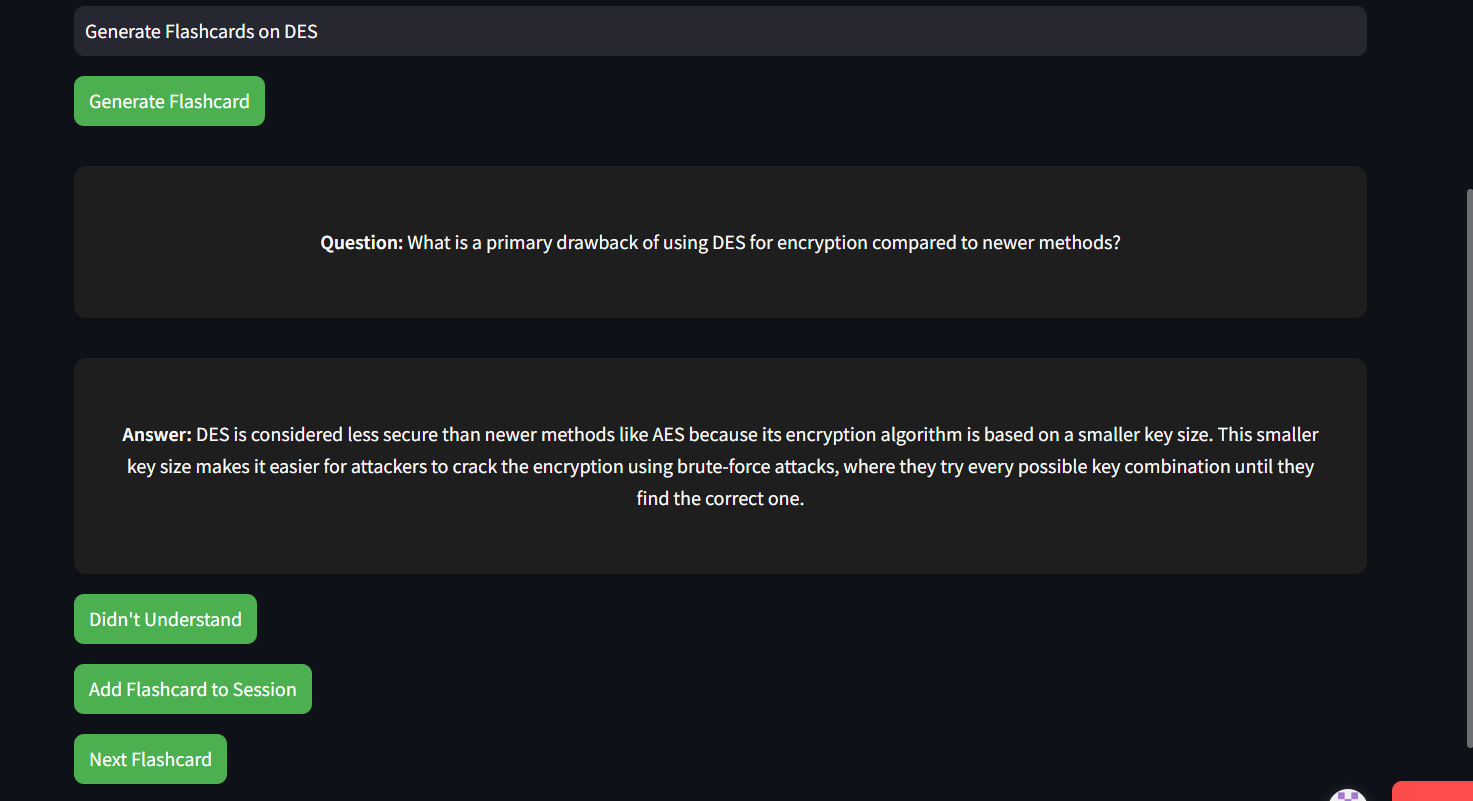
\includegraphics[width=0.9\textwidth]{flashcard-answer.png}
\caption{Flashcard Session - Answer}
\end{figure}
\begin{figure}[H]
\centering
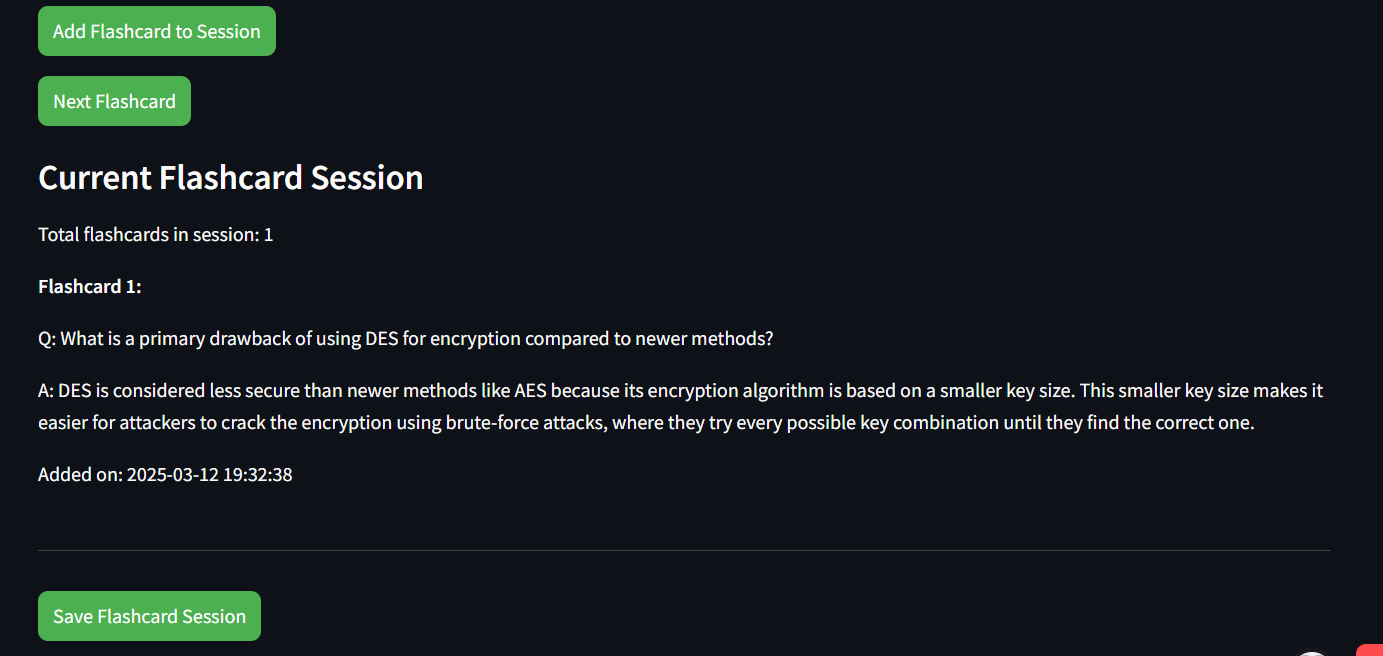
\includegraphics[width=0.9\textwidth]{saving-flashcard.png}
\caption{Flashcard Session - Saving}
\end{figure}
\begin{figure}[H]
\centering
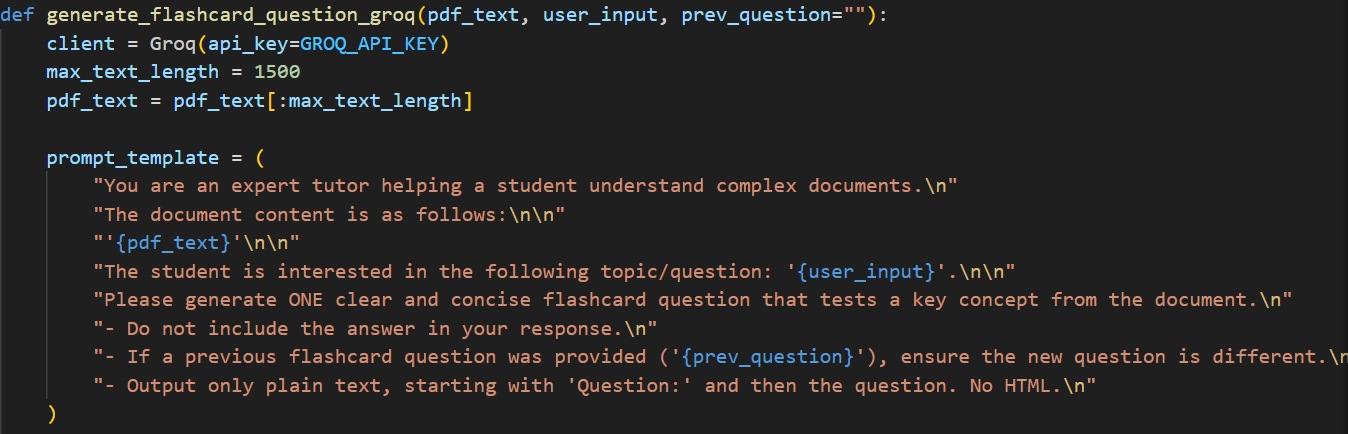
\includegraphics[width=0.9\textwidth]{flashcard-groq-code.png}
\caption{Flashcard Question Code Snippet}
\end{figure}
\begin{figure}[H]
\centering
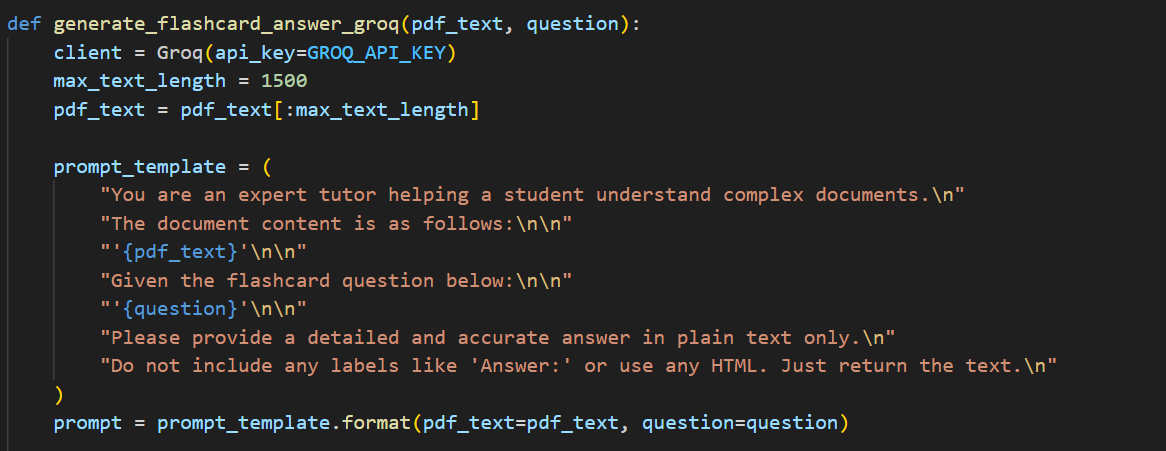
\includegraphics[width=0.9\textwidth]{flashcard-ans-groq-code.png}
\caption{Flashcard Answer Code Snippet}
\end{figure}
\begin{figure}[H]
\centering
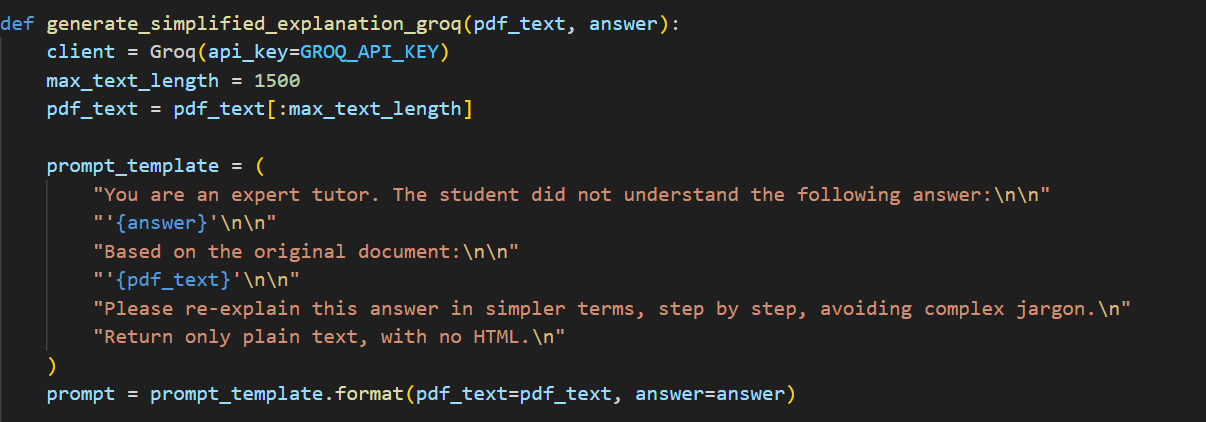
\includegraphics[width=0.9\textwidth]{simple-exp-code.png}
\caption{Flashcard Explanation Code Snippet}
\end{figure}

% Saved Flashcard Session
\subsection{Saved Flashcard Session}
Allows users to revisit previously saved flashcards.
\begin{figure}[H]
\centering
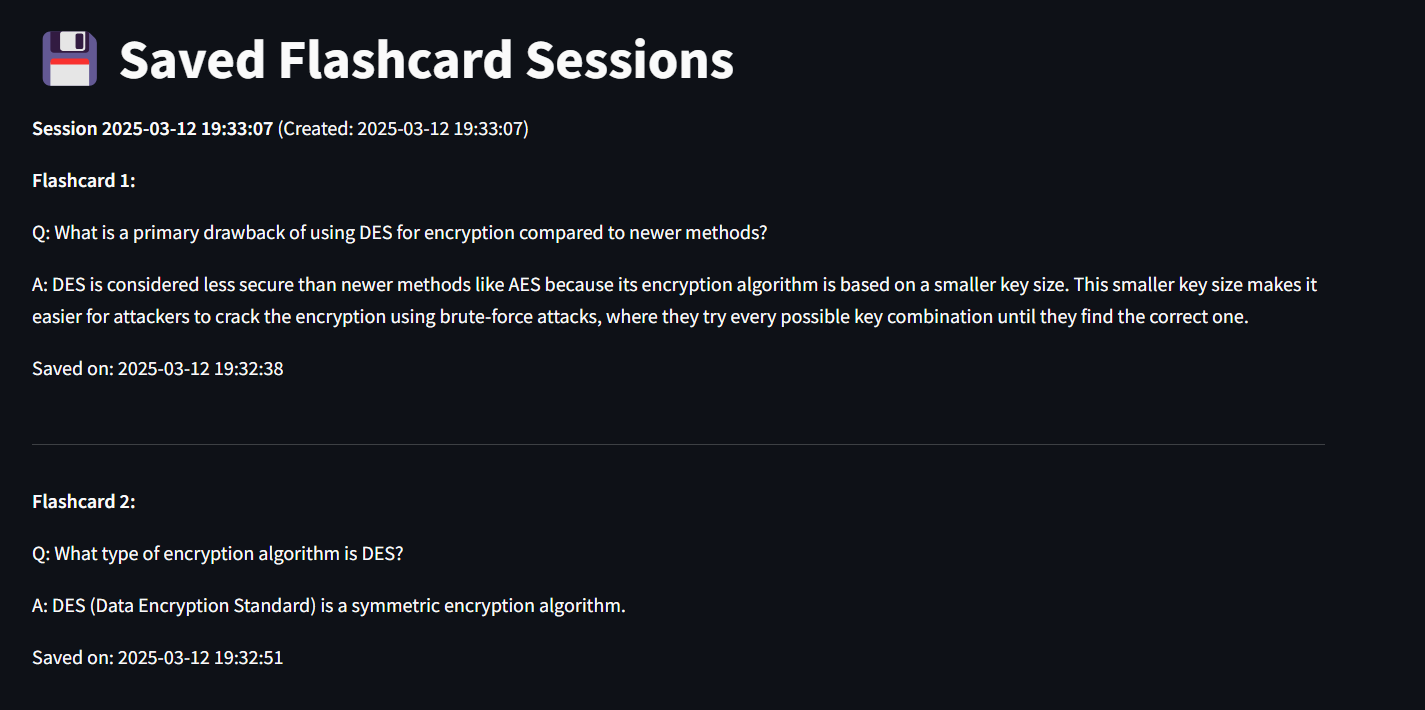
\includegraphics[width=0.9\textwidth]{saved-flashcard.png}
\caption{Saved Flashcards}
\end{figure}

% Test Session
\subsection{Test Session}
Engages users in quizzes and tests to reinforce learning.
\begin{figure}[H]
\centering
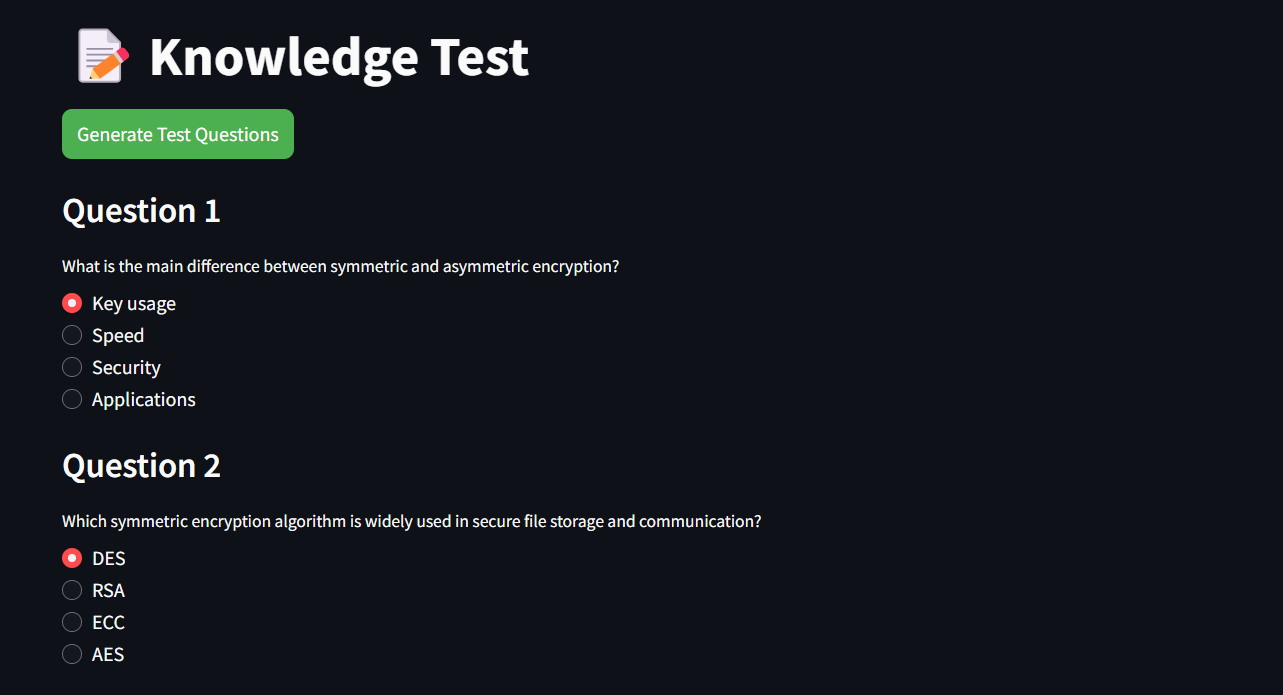
\includegraphics[width=0.9\textwidth]{test.png}
\caption{Test Session - Question}
\end{figure}
\begin{figure}[H]
\centering
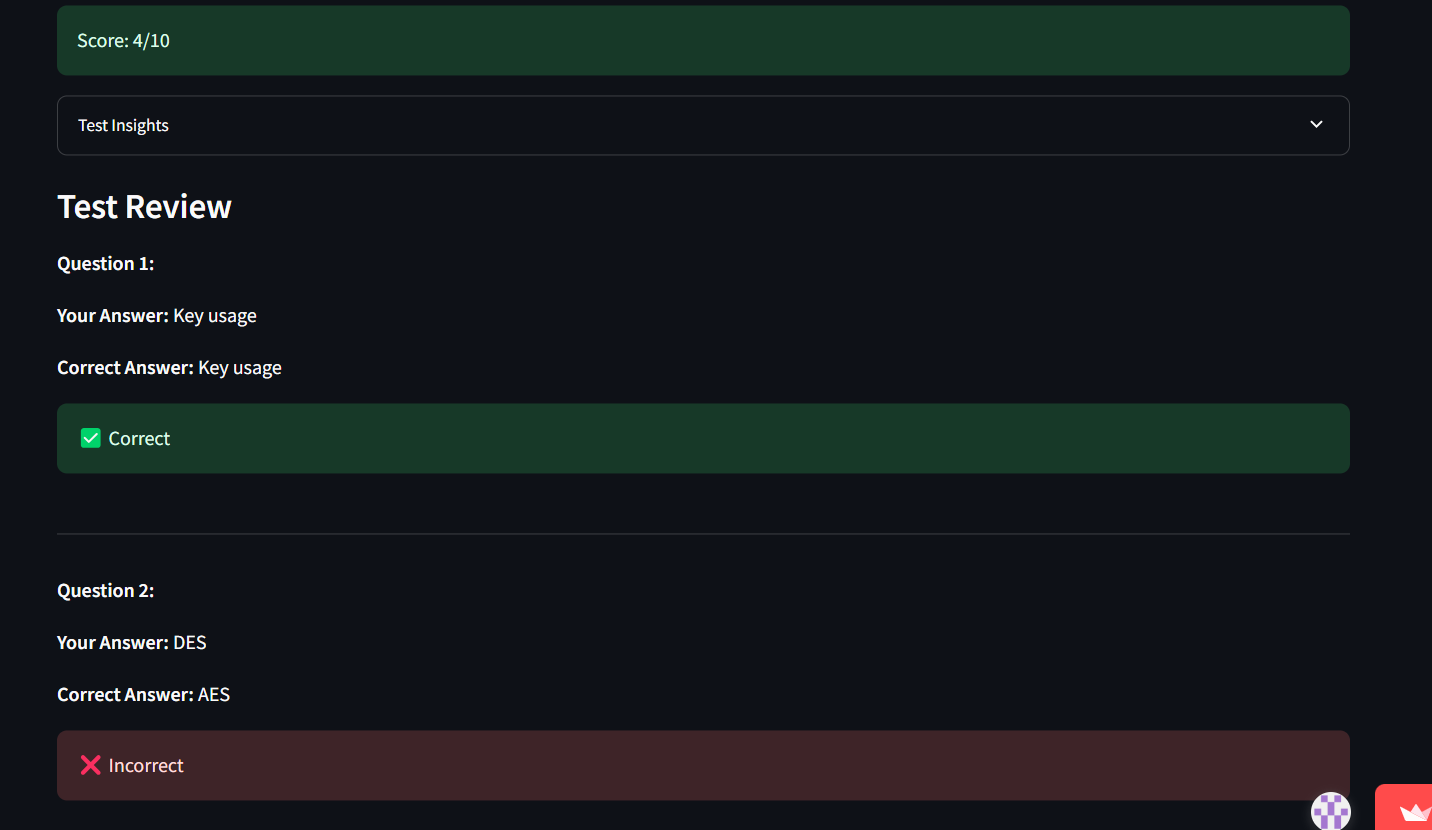
\includegraphics[width=0.9\textwidth]{test-score-result.png}
\caption{Test Session - Results}
\end{figure}
\begin{figure}[H]
\centering
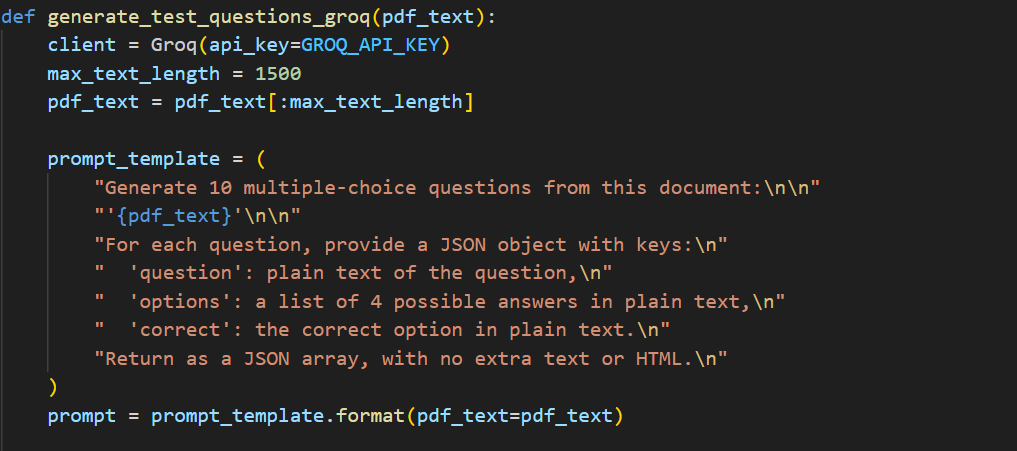
\includegraphics[width=0.9\textwidth]{test-code.png}
\caption{Test Code Snippet}
\end{figure}

% Community
\subsection{Community}
Facilitates interaction and collaboration among users.
\begin{figure}[H]
\centering
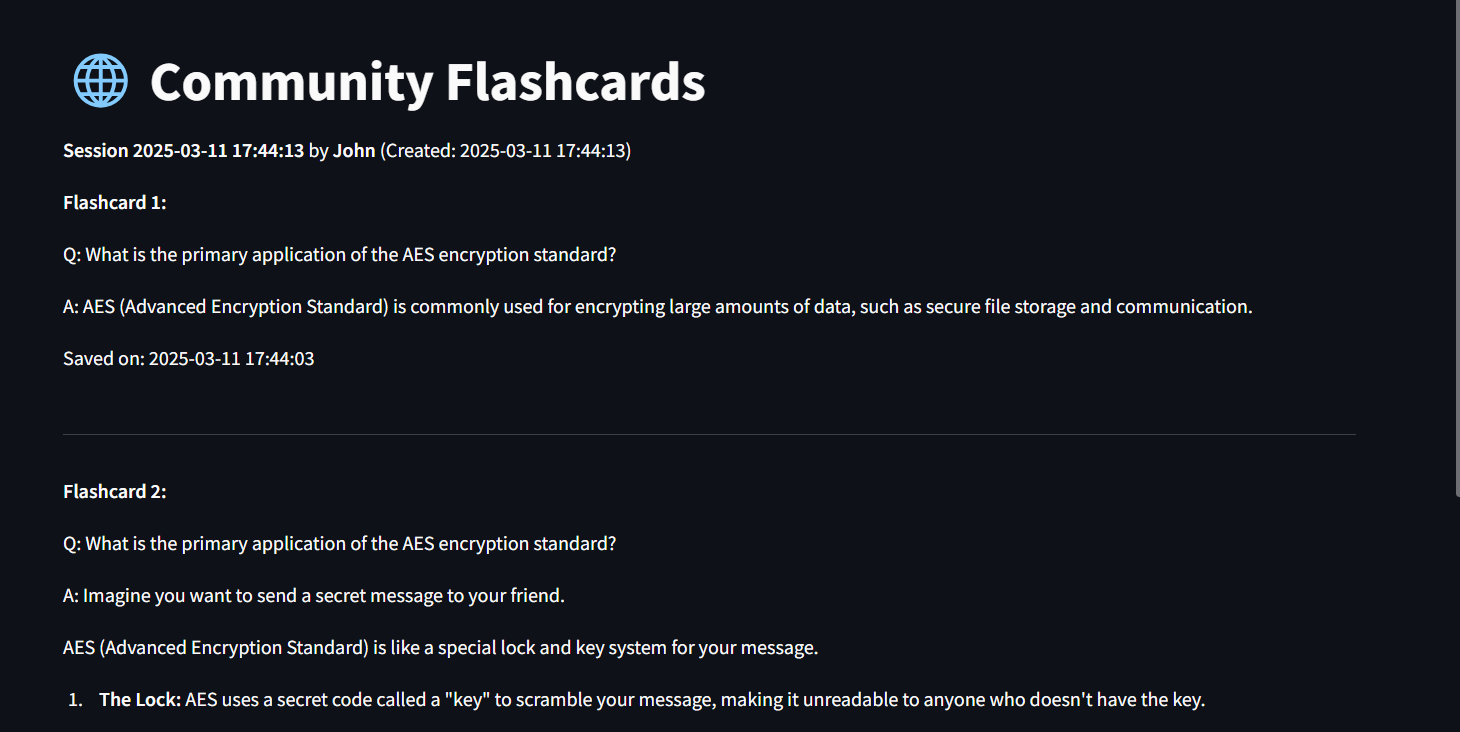
\includegraphics[width=0.9\textwidth]{community.png}
\caption{Community Features}
\end{figure}

% Test Insights
\subsection{Test Insights}
Provides detailed analytics and insights on user performance.
\begin{figure}[H]
\centering
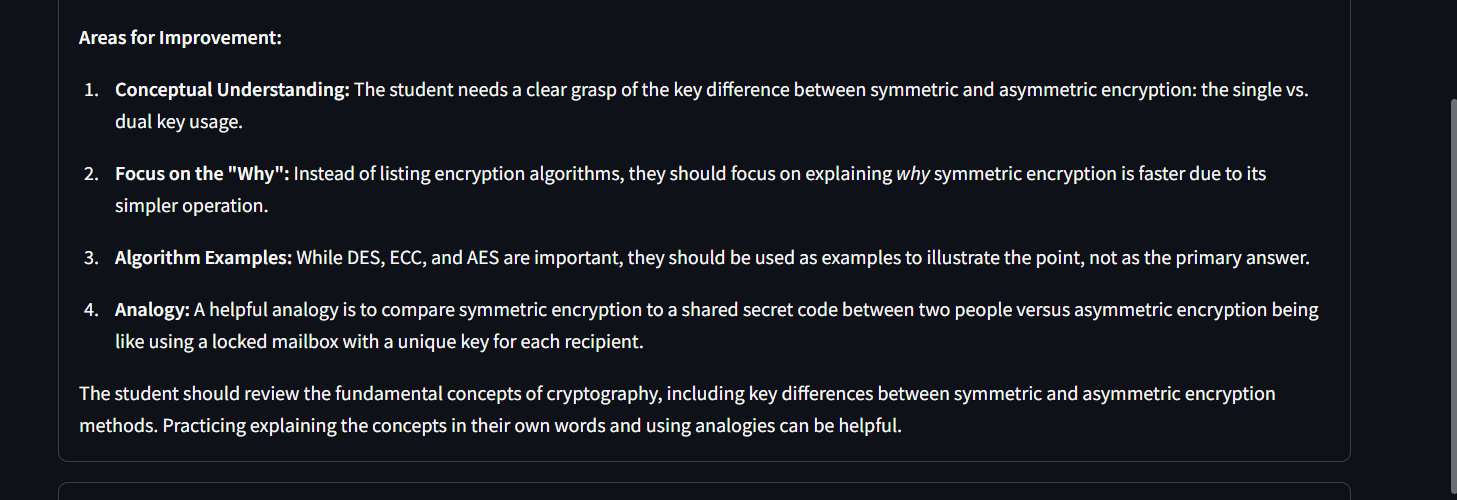
\includegraphics[width=0.9\textwidth]{test-insights.png}
\caption{Test Insights}
\end{figure}
\begin{figure}[H]
\centering
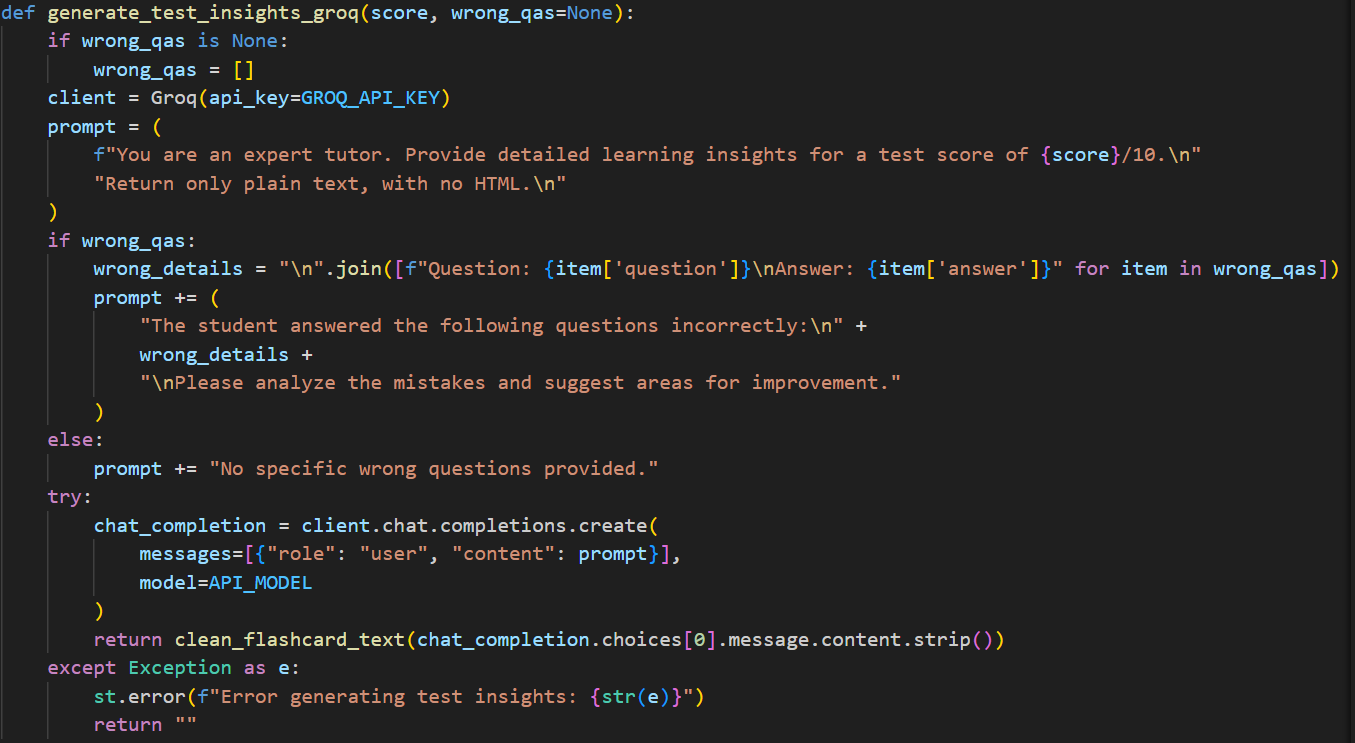
\includegraphics[width=0.9\textwidth]{test-insights-code.png}
\caption{Test Insights Code Snippet}
\end{figure}

% Graph and Table Section
\subsection{Graph and Table Section}
Displays data visualizations to track progress and performance.
\begin{figure}[H]
\centering
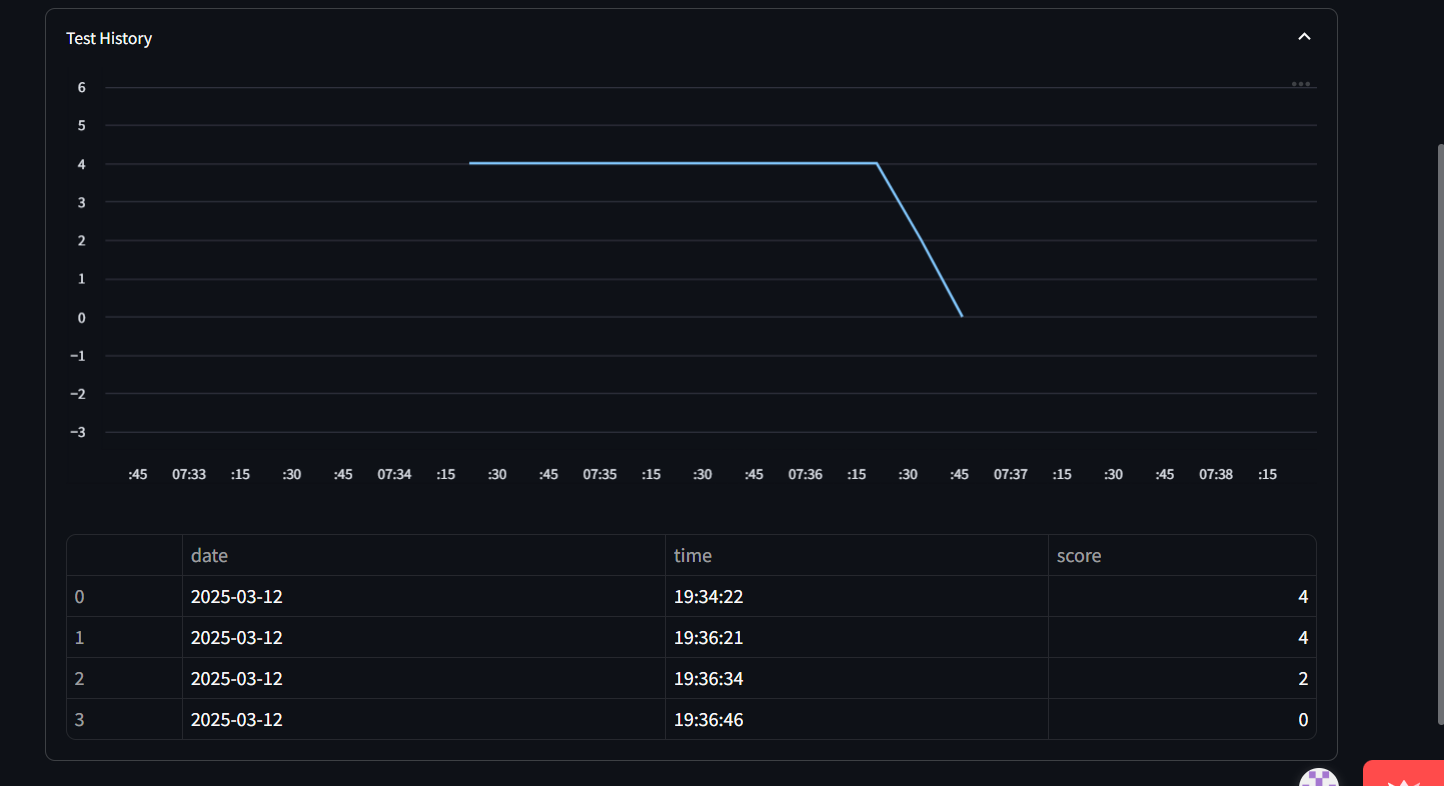
\includegraphics[width=0.9\textwidth]{graph-table.png}
\caption{Graphs and Tables}
\end{figure}
\begin{figure}[H]
\centering
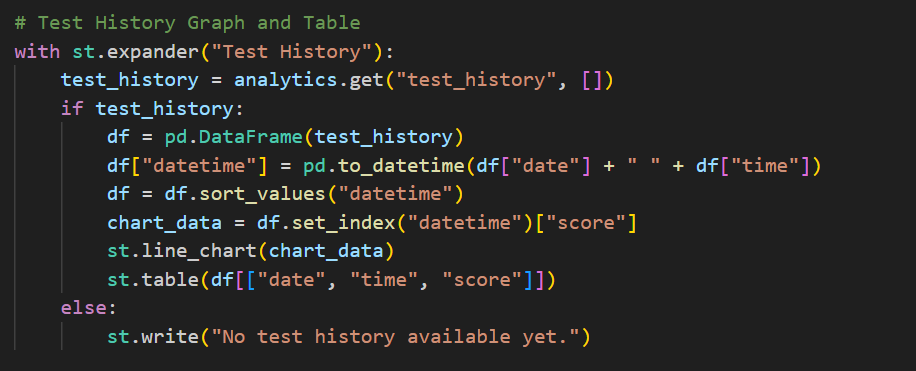
\includegraphics[width=0.9\textwidth]{graph-table-code.png}
\caption{Graph and Table Code Snippet}
\end{figure}

\section{Technology Stack}
\subsection{Frontend}
\begin{itemize}
    \item Streamlit for server-side rendering and client-side interactivity.
    \item Tailwind CSS for a responsive and modern UI.
    \item Recharts for data visualization in progress tracking.
\end{itemize}

\subsection{Backend}
\begin{itemize}
    \item Python and SQLite for API development.
    \item SQLite for data persistence.
    \item Auth0 for authentication and access control.
\end{itemize}

\subsection{AI and Machine Learning}
\begin{itemize}
    \item Groq API for natural language processing and flashcard generation.
    \item Python-based preprocessing scripts for text extraction.
\end{itemize}

\section{Deployment Strategy}
EduFlash is deployed using Vercel for frontend hosting and a cloud-based SQLite instance for the database. The backend API is hosted on a Python server with auto-scaling capabilities.

\section{Security Considerations}
\begin{itemize}
    \item Encrypted user authentication via Auth0.
    \item Secure API endpoints with token-based authentication.
    \item Data encryption for stored flashcards and user progress.
\end{itemize}

\section{Conclusion}
The implementation of EduFlash follows a structured, modular approach to ensure scalability, security, and effectiveness in delivering an interactive learning experience. Each component is optimized to work seamlessly, providing students with an efficient study tool tailored to their learning needs.


\chapter{Future Scope}

The future scope of EduFlash includes expanding its capabilities to support additional file formats such as EPUB and DOCX, enabling the use of a wider range of educational resources. As AI models continue to evolve, integrating more advanced algorithms could enhance content extraction and personalized learning, making the system even more adaptive.\\

Incorporating speech recognition and voice interaction could provide a more immersive, hands-free learning experience. Additionally, expanding support to multiple languages would increase accessibility for a global audience.\\

Future versions could also introduce collaborative learning features, allowing students to work together, share insights, and engage in peer reviews. Lastly, integrating real-time feedback, gamification elements, and personalized learning paths would further enhance motivation and engagement, creating a dynamic and interactive learning environment.

\chapter{Conclusion}

In conclusion, EduFlash is set to transform how students engage with educational content by converting textbooks into dynamic, personalized learning experiences. By integrating AI models like LLaMA and Gemini, the platform efficiently generates flashcards, quizzes, and adaptive learning pathways, ensuring effective comprehension of concepts.\\

As EduFlash evolves with emerging technologies and user feedback, it can expand to support various file formats, multilingual capabilities, and collaborative learning tools. These enhancements will cater to diverse learners, promoting a tailored educational experience.\\

The platform emphasizes engagement through interactive elements and real-time feedback, encouraging active participation and deeper understanding. Incorporating gamification techniques, such as rewards and challenges, can further motivate students, making learning enjoyable.Additionally, integrating analytics will provide educators with valuable insights into student progress, allowing for targeted instructional strategies.\\

Ultimately, EduFlash aims to foster a more engaging, efficient, and personalized learning environment for students globally. By bridging traditional education with modern technology, EduFlash is poised to make a significant impact on the future of learning, equipping students with essential skills for success in a rapidly evolving world.


\chapter{References}
\begin{itemize}
    \item Streamlit Documentation. (n.d.). Streamlit. \url{https://docs.streamlit.io/}
    \item SQLite Documentation. \url{https://www.sqlite.org/docs.html}
    \item Groq Documentation. \url{https://groq.com/docs}
    \item PyPDF2 Documentation. \url{https://pypdf2.readthedocs.io/en/latest/}
    \item Das, A., Malaviya, S., \& Singh, M. (2023). \textit{The Impact of AI-Driven Personalization on Learners' Performance}. International Journal of Computer Science and Education, 11(8), 1522. ISSN: 2347-2693
    \item Smith, J., \& Zhang, T. (2021). \textit{AI-based Automatic Flashcard Generation for Learning Enhancement}. Journal of Educational Technology, 48(3), 122-136.
    \item Ramteja Sajja, Yusuf Sermet, Muhammed Cikmaz, David Cwiertny, Ibrahim Demir. (2023). \textit{Artificial Intelligence-Enabled Intelligent Assistant for Personalized and Adaptive Learning in Higher Education}. University of Iowa.
    \item Patel, R., \& Liu, X. (2020). \textit{Leveraging NLP for Interactive Learning in Educational Platforms}. International Journal of Educational Computing Research, 36(4), 577-593.
    \item Riedel, S., Conneau, A., Cuturi, M., \& LeCun, Y. (2020). \textit{Retrieval-Augmented Generation for Knowledge Intensive NLP Tasks}. NeurIPS 2020.
\end{itemize}





\end{document}
